\section{Pressure-coefficient distribution along the RDT blade}
\label{sec:methods_rdt_cp}
 
In addition to the velocity-triangle characterisation in
Section~\ref{sec:methods_rdt_velocity_triangles}, the converged RDT-only
solution is post-processed for the pressure distribution along the
rotor blade contour at eleven radial spans, $r/R\in\{0.01,\,0.10,\,
0.20,\,0.30,\,\ldots,\,0.90,\,0.99\}$. The data are exported as
blade-loading lines that traverse the blade contour
$\mathrm{LE}\to\mathrm{SS}\to\mathrm{TE}\to\mathrm{PS}\to\mathrm{LE}$,
where SS denotes the suction side and PS the pressure side. The
streamwise coordinate $s\in[0,1]$ is normalised along the chord. Both
surfaces appear naturally as the two branches of the same continuous
contour line.
 
\paragraph{Pressure-coefficient definition.}
The static pressure $p$ is non-dimensionalised at each radius by the
dynamic pressure based on the local blade speed,
%
\begin{equation}
C_p(s,\,r) \;=\; \frac{p(s,\,r) - p_{\mathrm{ref}}}
                       {\frac{1}{2}\,\rho\,U^{2}(r)},
\qquad
U(r) \;=\; \omega\,r,
\label{eq:Cp_definition}
\end{equation}
%
where $\omega$ is the rotor angular velocity and $\rho$ the water
density. The reference pressure $p_{\mathrm{ref}}$ is the median
pressure across all spans and all chord positions of the converged
solution; this is a robust free-stream-like reference that makes the
$C_p$ profiles directly comparable across spans without privileging any
single radial location. With this scaling, $C_p$ is bounded near $-1$
and $+1$ in the inner-mid-span region for a well-formed pump rotor, and
positive (negative) values indicate static pressure above (below) the
reference.
 
\paragraph{Distribution at eleven spans.}
Figure~\ref{fig:rdt_cp_distribution} shows $C_p(s)$ for all eleven
spans, grouped by radial position into a hub-region panel
($r/R\leq 0.30$), a mid-span panel ($0.40\leq r/R\leq 0.70$), and a
tip-region panel ($r/R\geq 0.80$). Three distinct regimes are visible.
 
\begin{figure}[H]
  \centering
  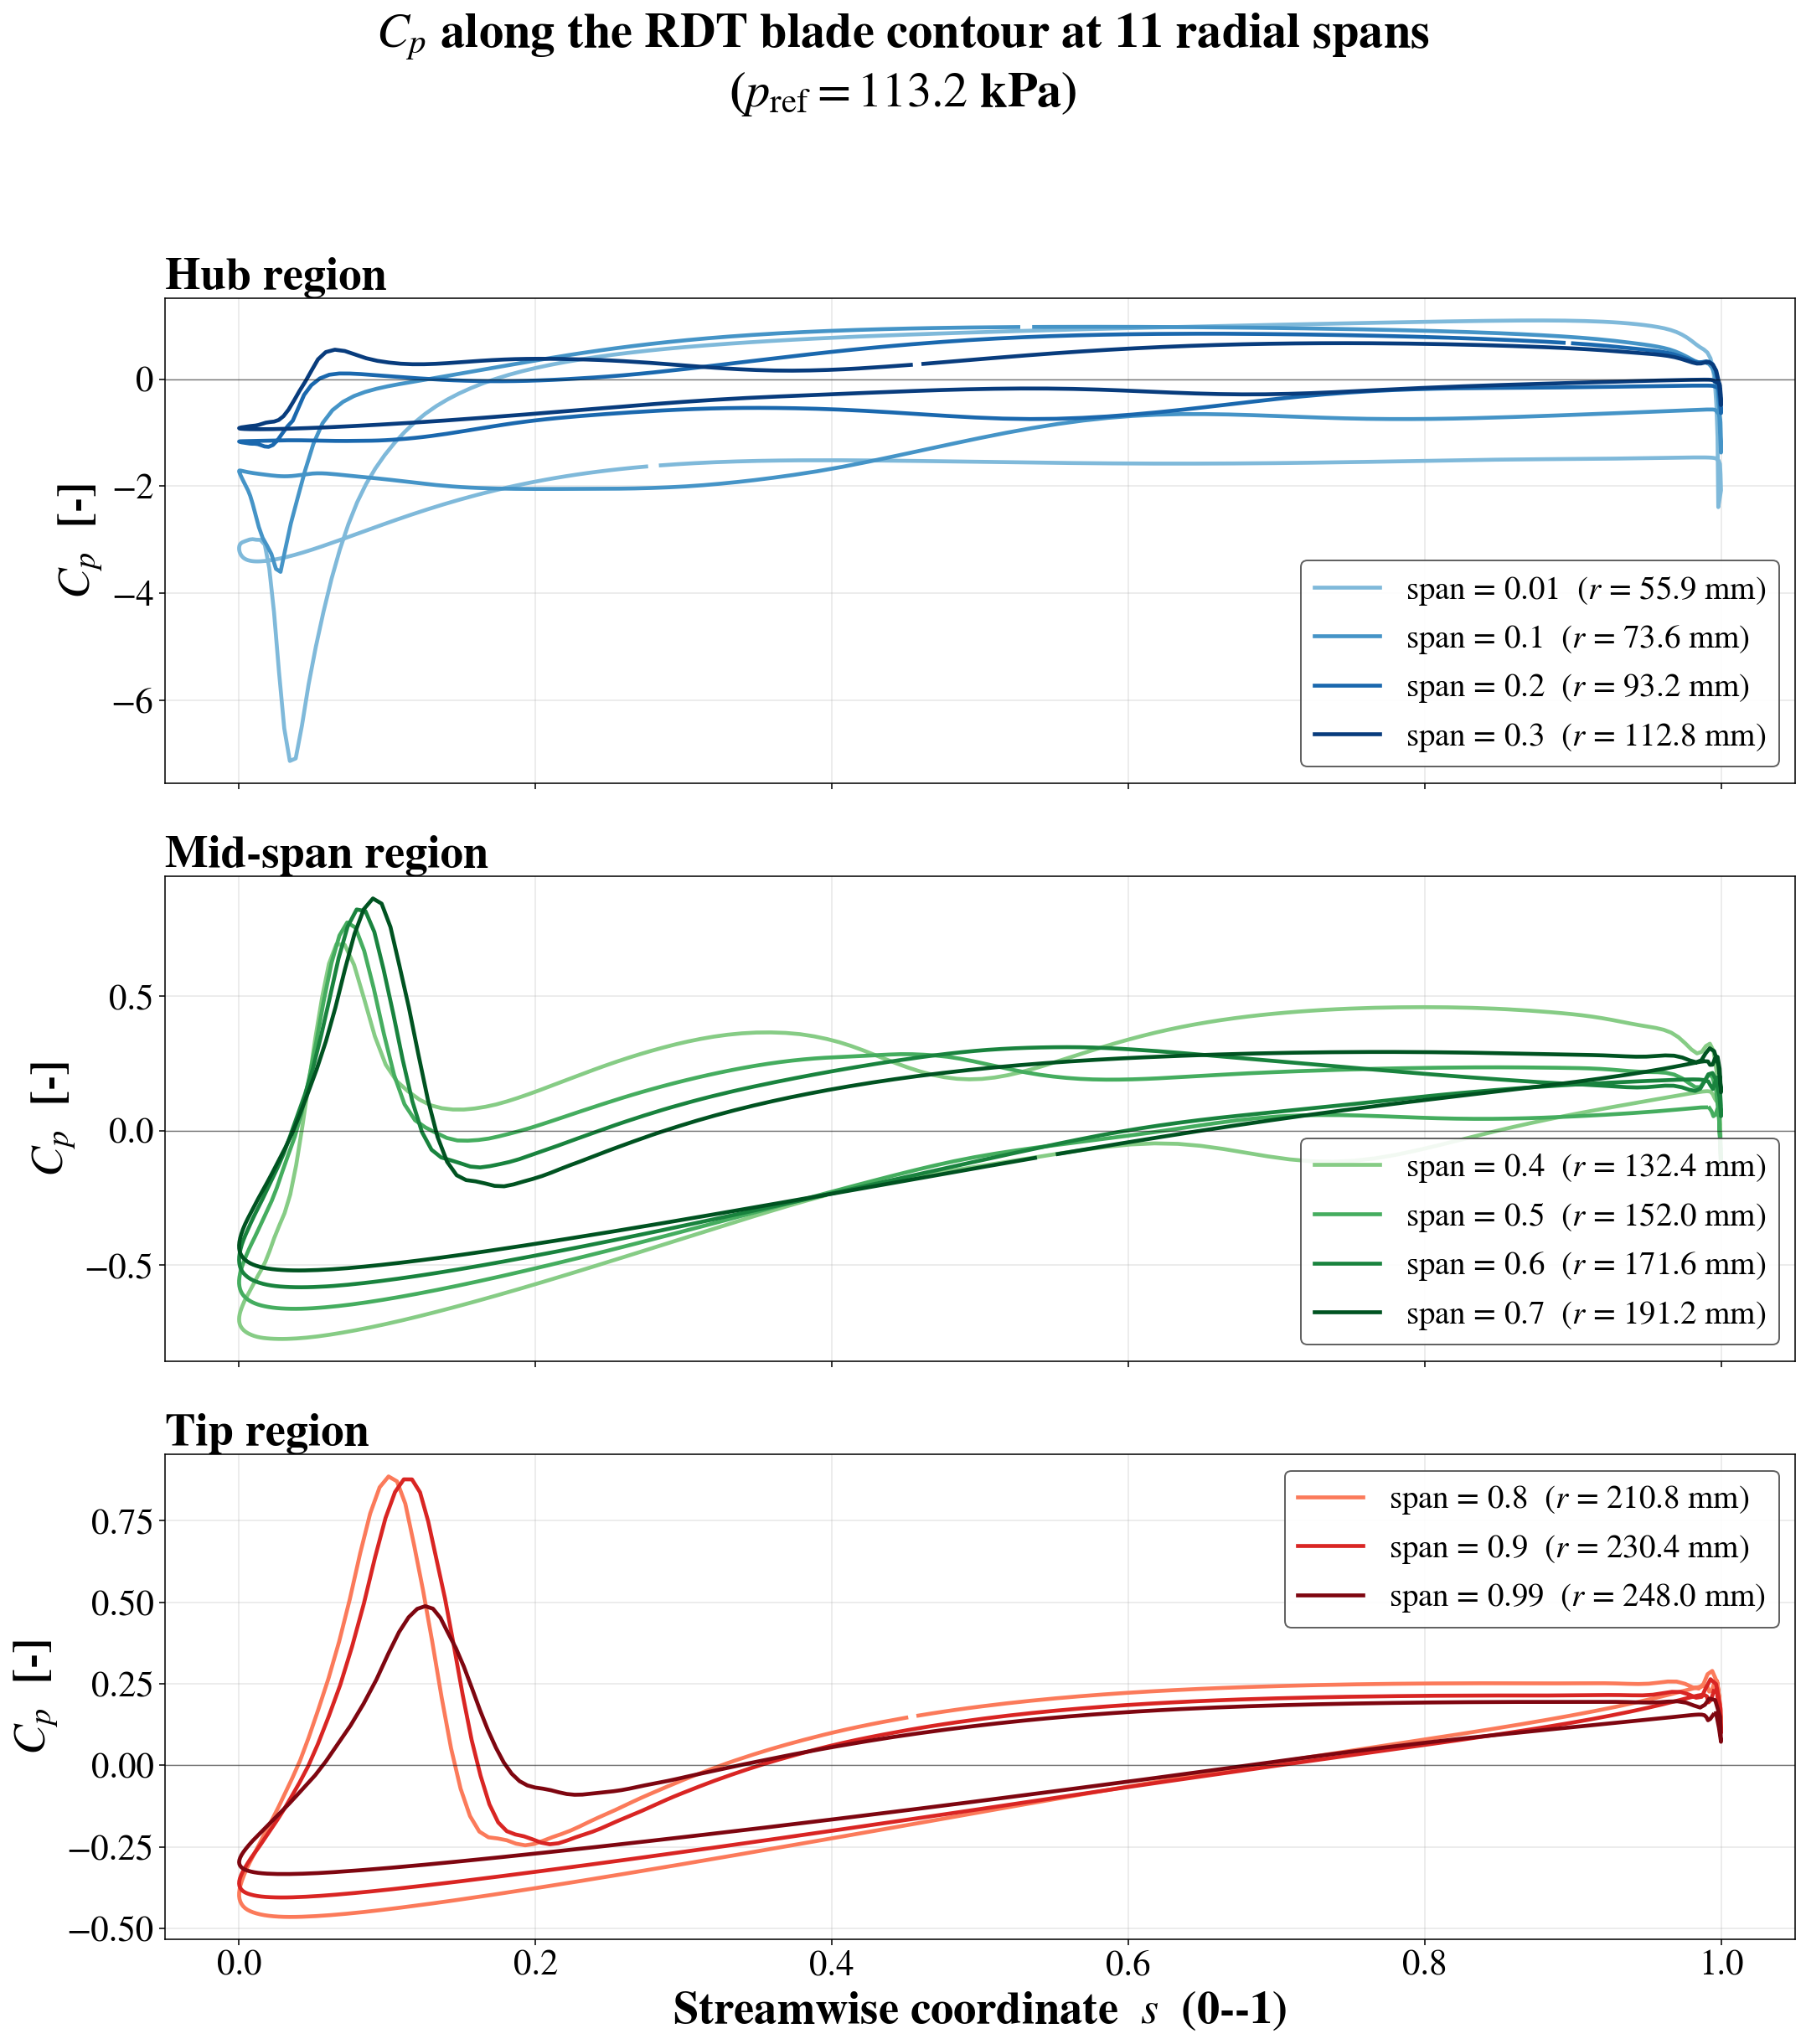
\includegraphics[width=\linewidth]{Figures/RDT/Spanwise_Cp_RDT.png}
  \caption[Pressure-coefficient distribution along the RDT blade]
  {Pressure coefficient $C_p$ along the RDT blade contour at eleven
  radial spans. Each curve is a single continuous traversal of the
  blade contour
  $\mathrm{LE}\to\mathrm{SS}\to\mathrm{TE}\to\mathrm{PS}\to\mathrm{LE}$;
  the two visible branches at every $s$ correspond to the suction
  side (lower $C_p$) and the pressure side (higher $C_p$). The
  reference pressure is the median pressure across all spans,
  $p_{\mathrm{ref}}=113.2$~kPa. The grouping is hub
  ($r/R\leq 0.30$, top), mid-span ($0.40\leq r/R\leq 0.70$, middle),
  and tip ($r/R\geq 0.80$, bottom). The hub panel uses a different
  vertical scale than the mid-span and tip panels because of the
  large suction peak at $r/R=0.01$.}
  \label{fig:rdt_cp_distribution}
\end{figure}
 
\paragraph{Hub region (top panel).}
The innermost station, $r/R=0.01$, exhibits a deep suction peak with
$C_p\approx -7$ near $s\approx 0.05$ and an essentially absent
pressure-side loading. This indicates strong local acceleration around
the blade leading edge in the immediate hub vicinity, consistent with
high local incidence and with the absence of an actual hub solid body
in this hubless rim-driven thruster~\cite{Verdijck2025}. Moving outward
to $r/R=0.10,\,0.20$ and $0.30$, the suction peak weakens rapidly and
the pressure side becomes increasingly identifiable, but a clean
PS--SS separation is only consistently established from
$r/R\gtrsim 0.30$ onwards. The hub region is therefore the part of the
RDT outflow where the blade-loading concept itself is least
representative of an aerofoil-like cascade. This observation is
consistent with the backflow-dominated rings identified at
$r<0.12$~m in the convergence analysis of
Section~\ref{sec:methods_rdt_baseline_alpha} and provides a physical
justification for the inner cut-out at $r=0.12$~m used in the
guide-vane design span: the hub region delivers a flow that is
dominated by recirculation rather than by a coherent rotor wake that
the guide vanes can usefully condition.
 
\paragraph{Mid-span region (middle panel).}
The four mid-span stations, $r/R\in\{0.40,\,0.50,\,0.60,\,0.70\}$,
display the classical pump-rotor blade-loading shape. The pressure side
exhibits a localised peak of $C_p\approx +0.7$--$+0.9$ near
$s\approx 0.10$, the suction side reaches a minimum of
$C_p\approx -0.5$--$-0.7$ at the same chord location, and both surfaces
recover smoothly through the diffusion region towards a near-zero
$C_p$ at the trailing edge. The PS--SS separation is well-defined and
the loading area enclosed between the two branches is large, indicating
that this part of the blade does most of the useful pumping work. The
absence of a flat or rising suction-side recovery suggests that no
significant boundary-layer separation develops on the SS in the
mid-span region under the present design point.
 
\paragraph{Tip region (bottom panel).}
At $r/R\in\{0.80,\,0.90\}$ the qualitative shape of the loading is the
same as the mid-span, but the suction peak intensifies further with
radius. The peak suction-side magnitude reaches $C_p\approx -0.4$ and
the peak pressure-side value rises to $C_p\approx +0.9$ at
$r/R=0.80$--$0.90$, which is consistent with the larger blade speed
$U(r)=\omega r$ at the outer span and with the higher local relative
velocity. At the outermost station, $r/R=0.99$, however, the loading
drops noticeably: the PS--SS branches collapse towards each other and
the enclosed loading area shrinks. The tip-vortex flow and the
finite tip-clearance treatment unload the blade locally, in a manner
that is well documented for ducted thrusters and pump
rotors~\cite{Verdijck2025}. This unloading produces the
characteristic outer-radius dip in $\alpha(r)$ that the baseline
construction in
Section~\ref{sec:methods_rdt_baseline_alpha} replaces with a
$60^\circ$ plateau, since designing the guide-vane outer-span metal
angle against this tip-driven feature would couple the vane geometry
to a feature of the rotor that is not part of the swirl pattern the
guide-vane row is intended to recover.
 
\paragraph{Implications for the guide-vane design.}
Three implications follow from Figure~\ref{fig:rdt_cp_distribution} and
are used in the GV-design choices made in
Section~\ref{sec:methods_design_matrix}. First, the breakdown of the
blade-loading concept at $r/R\lesssim 0.20$ supports the choice of an
inner cut-out at $r=0.12$~m: there is no coherent rotor outflow inside
that radius for the guide vanes to recover. Second, the existence of a
clean PS--SS pump-rotor loading from $r/R\gtrsim 0.30$ outward confirms
that the swirl distribution $C_u(r)$ obtained from the converged plane
is generated by a healthy, well-attached rotor and is not an artefact
of off-design separation; the spanwise design input
$(C_m(r),\,C_u(r))$ is therefore a meaningful target for the guide-vane
generator. Third, the tip-vortex unloading at $r/R\approx 0.99$
provides the physical justification for the plateau-bounded baseline
$\alpha_{\mathrm{base}}(r)$ used in
Section~\ref{sec:methods_rdt_baseline_alpha}: the local outer-radius
dip in $\alpha(r)$ originates in the tip-clearance flow rather than in
the bulk wake, and the guide-vane row should not be designed to track
it.

% \chapter{Design Methodology}
% \label{chap:chap4}

% % ---------------------------------------------------------------------
% \section{Overview of the methodology}
% \label{sec:methods_overview_master}
 
% The methodology of this thesis combines a parametric MATLAB tool that generates 24 candidate guide-vane geometries, a multi-domain ANSYS~CFX setup that simulates each configuration in the full RDT--GV--draft-tube layout under identical operating conditions, and a structured post-processing pipeline that extracts a common set of metrics on a fixed array of analysis planes. The MATLAB tool is the same tool developed in the project work~\cite{Leonsen2025}; its operating principle is briefly recalled here and is not redeveloped from scratch. The CFX setup, in contrast, is specific to the present thesis: the draft-tube domain has been extended to include the conical contraction, the $90^\circ$ bend and a final straight inlet pipe, and the boundary conditions reflect the full nominal operating point at $\dot m = 290.3$~kg/s and $n = 650$~rpm.
 
% Figure~\ref{fig:methodology_overview} summarises the workflow. Each branch of the design matrix (Section~\ref{sec:methods_design_matrix}) goes through the same pipeline: section generation in MATLAB, three-dimensional lofting in the Visual-Studio CAD tool inherited from the project work, blade meshing in ANSYS TurboGrid, integration with the structured RDT mesh and the unstructured downstream-duct mesh, simulation in ANSYS~CFX, and post-processing on the common plane array.
 
% \begin{figure}[h!]
%   \centering
%   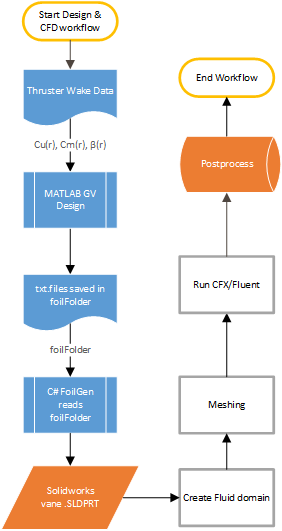
\includegraphics[width=0.6\textwidth]{Figures/FlowChart/Full_flowchart.png}
%   \caption[Methodology overview]{Methodology overview for the 24-case screening campaign. Each configuration follows the same pipeline from MATLAB section generation to CFX simulation and post-processing.}
%   \label{fig:methodology_overview}
% \end{figure}
 
% % ---------------------------------------------------------------------
% \section{Parametric guide-vane design tool}
% \label{sec:methods_matlab_tool}
 
% The guide-vane geometries are generated by the MATLAB tool \texttt{vanedesign\_loft\_export.m} that was developed in the project work~\cite{Leonsen2025}. The tool reads spanwise distributions $\{r,\,C_m(r),\,C_u(r)\}$ from the RDT wake, computes the local inlet flow angle $\beta_1(r) = \arctan(C_u/C_m)$ and the local diameter-based Reynolds number $\mathrm{Re}_D(r)$, and then constructs the metal angles, chord distribution, two-dimensional camber and thickness, and the three-dimensional wrapped vane surface. The geometric construction is described in Section~\ref{sec:theory_geometric_construction} of the theory chapter. The output of the tool is an STL file together with a set of section curves that can be imported by the Visual-Studio CAD tool inherited from~\cite{Verdijck2025} and lofted into a CFD-ready solid.
 
% The tool exposes a structured options list, of which the following are exercised in the screening campaign:
% \begin{itemize}
%   \item \texttt{Zs}: vane count;
%   \item \texttt{use\_sigma}: boolean switching between fixed chord (\texttt{false}) and target solidity (\texttt{true});
%   \item \texttt{c\_const\_fallback}: shroud chord when \texttt{use\_sigma = false};
%   \item \texttt{sigma\_target}: target solidity at the shroud when \texttt{use\_sigma = true};
%   \item \texttt{slip\_choice = 'const'} with \texttt{slip\_const\_deg = 6.0}: fixed slip correction in line with G\"ulich's recommendation~\cite{Gulich2010};
%   \item \texttt{tc\_rel = 0.075}, \texttt{tTE\_rel = 0.005}, \texttt{LE\_round = 1.2}: thickness law parameters held constant;
%   \item \texttt{use\_cone\_wrap = false}, \texttt{use\_TE\_anchor = true}: cylindrical wrapping with a common trailing-edge azimuth;
%   \item \texttt{lean\_amp = 0}, \texttt{sweep\_amp = 0}: lean and sweep held at zero in the screening campaign.
% \end{itemize}
 
% \paragraph{Choice of slip-correction strategy.}
% The project work~\cite{Leonsen2025} developed a CFD-based slip database and a smooth response-surface model that predicts deviation as a function of inlet flow angle and Reynolds number. At the high turning angles required to recover the RDT swirl, this response surface predicts deviation values on the order of $10^\circ$--$20^\circ$. Adopting these large built-in trailing-edge angles aggressively over-cambers the section near the trailing edge, sharpens the suction-side adverse pressure gradient, and tends to promote separation. The classical recommendation by G\"ulich~\cite{Gulich2010} is more conservative: a small built-in angle of approximately $4^\circ$--$6^\circ$ is sufficient to compensate for cascade deviation in well-designed pump and stator vanes. The present screening campaign adopts the upper end of this range, $\delta_{\mathrm{TE}} = 6^\circ$, applied as a constant correction to the trailing-edge metal angle for every section across all 24 configurations. This choice reduces one degree of freedom in the screening campaign and isolates the chord-strategy and vane-count effects that the master thesis is designed to study. The trade-off between aggressive slip correction (response surface) and conservative slip correction (G\"ulich) is acknowledged as a question that could be revisited in a focused follow-up study using a small subset of the screening configurations.
 
% \paragraph{Spanwise inlet data.}
% The spanwise distributions $\{r,\,C_m(r),\,C_u(r)\}$ used as the design input are taken from the recent RDT simulations \texttt{shubham\_blade6} and \texttt{shubham\_transient} carried out by Sharma and Djupesland (referenced via~\cite{Leonsen2025}), evaluated at a plane $0.25$~m downstream of the rotor. The valid design span is restricted to radii with positive meridional velocity. As discussed in Section~\ref{sec:theory_backflow_span}, this corresponds approximately to $r \in [0.12, 0.25]$~m, which is the radial extent of all guide vanes used in the screening campaign.
 
% % ---------------------------------------------------------------------
% \section{Design matrix: 24 configurations}
% \label{sec:methods_design_matrix}
 
% The design space is sampled on a structured matrix of 24 configurations that combines two design strategies, four shroud-chord levels and two to three vane counts. The case-naming convention used throughout this thesis is
 
% \medskip
% \centerline{\texttt{<strategy>\_<chord shroud in mm>\_<Z\_s>}}
% \medskip
 
% \noindent
% where \texttt{strategy} is either \texttt{CC} (constant chord) or \texttt{CS} (constant solidity at the shroud), the second field is the chord at the shroud in millimetres, and the third field is the vane count $Z_s$. For example, \texttt{CC\_400\_8} denotes a constant-chord configuration with $c = 400$~mm at all radii and $Z_s = 8$ vanes, while \texttt{CS\_400\_8} denotes a constant-solidity configuration that has $c(r=0.25) = 400$~mm at the shroud, scaling chord linearly with $r$ inwards to keep solidity constant. The full list of 24 configurations is given in Table~\ref{tab:design_matrix}.
 
% \begin{table}[h!]
%   \centering
%   \caption[24-case design matrix]{Design matrix used in the screening campaign. CC denotes constant chord, CS denotes constant solidity referenced at the shroud. All configurations are simulated at $\dot m = 290.3$~kg/s and $n = 650$~rpm with the same RDT inlet wake and the same downstream draft-tube geometry.}
%   \label{tab:design_matrix}
%   \small
%   \begin{tabular}{l|c|c|c}
%     \toprule
%     \textbf{Case ID} & \textbf{Strategy} & $c_{\mathrm{shroud}}$ (mm) & $Z_s$ \\
%     \midrule
%     CC\_250\_6  & Constant chord    & 250 & 6 \\
%     CC\_250\_8  & Constant chord    & 250 & 8 \\
%     CC\_250\_9  & Constant chord    & 250 & 9 \\
%     CC\_300\_6  & Constant chord    & 300 & 6 \\
%     CC\_300\_8  & Constant chord    & 300 & 8 \\
%     CC\_300\_9  & Constant chord    & 300 & 9 \\
%     CC\_350\_6  & Constant chord    & 350 & 6 \\
%     CC\_350\_8  & Constant chord    & 350 & 8 \\
%     CC\_400\_6  & Constant chord    & 400 & 6 \\
%     CC\_400\_8  & Constant chord    & 400 & 8 \\
%     CC\_450\_6  & Constant chord    & 450 & 6 \\
%     CC\_450\_7  & Constant chord    & 450 & 7 \\
%     CC\_450\_8  & Constant chord    & 450 & 8 \\
%     \midrule
%     CS\_250\_6  & Constant solidity & 250 & 6 \\
%     CS\_250\_8  & Constant solidity & 250 & 8 \\
%     CS\_250\_9  & Constant solidity & 250 & 9 \\
%     CS\_300\_6  & Constant solidity & 300 & 6 \\
%     CS\_300\_8  & Constant solidity & 300 & 8 \\
%     CS\_300\_9  & Constant solidity & 300 & 9 \\
%     CS\_350\_6  & Constant solidity & 350 & 6 \\
%     CS\_350\_8  & Constant solidity & 350 & 8 \\
%     CS\_400\_6  & Constant solidity & 400 & 6 \\
%     CS\_400\_8  & Constant solidity & 400 & 8 \\
%     CS\_450\_8  & Constant solidity & 450 & 8 \\
%     \bottomrule
%   \end{tabular}
% \end{table}
 
% \paragraph{Coverage and rationale.}
% The matrix covers the four shroud-chord levels $\{250, 300, 350, 400, 450\}$~mm and the vane counts $\{6, 7, 8, 9\}$, with combinations chosen to give roughly balanced coverage of the loading regime. Constant-chord cases probe the situation where the inner span carries proportionally more loading than the outer span; constant-solidity cases probe the situation where loading is uniform across the span at the cost of more wetted area. Within each strategy, the variation in shroud chord and vane count spans approximately a factor of two in solidity at the shroud, which is sufficient to map the trade-off between swirl reduction and total-pressure loss without overstretching the available CFD time. Cases that lie close to expected boundaries of the trade-off, e.g.\ very low solidity at high $Z_s$ that would behave essentially as a high-loss screen, are deliberately excluded.
 
% \paragraph{Constants across the matrix.}
% All 24 configurations share the following constants, so that the only differences between cases are the design variables stated in Table~\ref{tab:design_matrix}: thickness ratio $(t/c)_{\mathrm{rel}} = 0.075$; trailing-edge thickness $t_{\mathrm{TE}}/c = 0.005$; leading-edge roundness factor $\texttt{LE\_round} = 1.2$; slip correction $\delta_{\mathrm{TE}} = 6^\circ$; cylindrical wrapping; trailing-edge anchoring at a common azimuth; design span $r \in [0.12, 0.25]$~m. Operating conditions are also held fixed: $\dot m = 290.3$~kg/s, $n = 650$~rpm, water at standard laboratory conditions.
 
% % ---------------------------------------------------------------------
% \section{Computational domain and boundary conditions}
% \label{sec:methods_domain}
 
% The computational domain reproduces the planned Store2Hydro layout from the RDT inlet down to the location where the RPT inlet would be. Six contiguous regions are connected through stationary--stationary or rotating--stationary interfaces. The domain is sketched schematically in Figure~\ref{fig:domain_master_overview} and the regions are listed in Table~\ref{tab:domains}.
 
% \begin{table}[h!]
%   \centering
%   \caption[Domain regions]{Regions of the multi-domain CFX setup, in flow direction.}
%   \label{tab:domains}
%   \small
%   \begin{tabular}{c|l|l}
%     \toprule
%     \textbf{Region} & \textbf{Description} & \textbf{Mesh tool} \\
%     \midrule
%     1 & Inlet pipe, $D = 0.5$~m, length $0.5$~m   & ANSYS Meshing (unstructured) \\
%     2 & RDT rotor, $Z_r = 7$ blades              & ANSYS TurboGrid (structured) \\
%     3 & Guide-vane row (case-dependent)          & ANSYS TurboGrid (structured) \\
%     4 & Inner-pipe section, $r < 0.12$~m         & ANSYS Meshing (structured hub) \\
%     5 & Conical contraction, $D = 0.5 \to 0.4$~m & ANSYS Meshing (unstructured) \\
%     6 & Draft tube: $90^\circ$ bend + final straight pipe ($\sim 1.0$~m) & ANSYS Meshing (unstructured) \\
%     \bottomrule
%   \end{tabular}
% \end{table}
 
% \paragraph{Reasons for the extended draft-tube length.}
% The final straight pipe in region 6 is approximately $1.0$~m long and replaces the RPT in the present screening study. Two reasons motivate this choice. First, simulating the coupled RDT--GV--RPT system at the scale of 24 configurations was estimated to exceed the available computational budget by approximately a factor of three; the parallel project~\cite{Dokset2025} carries the responsibility for the RPT side. Second, an extended straight pipe creates a buffer between the bend exit and the imposed outlet boundary condition. Without this buffer, the imposed static-pressure outlet would project upstream and contaminate the post-bend flow field that is used to evaluate the residual swirl and the post-bend uniformity. With a $\sim 1.0$~m straight buffer, the flow has approximately $2.5$ duct diameters to redevelop after the bend before it reaches the outlet plane, which experience from comparable configurations indicates is sufficient to suppress upstream contamination of the analysis planes within a few percent in the integral metrics~\cite{Xia1997}.
 
% \paragraph{Limitation: absence of the RPT suction effect.}
% The RPT in pump mode draws fluid through its runner, and the suction field of the runner influences the upstream draft-tube velocity profile. This suction effect is not represented in the present setup, where the RPT is replaced by an extended straight pipe. The present study therefore does not predict absolute RPT-side performance and cannot be compared directly with operating measurements of the full machine. What the study does predict, and what it is designed to predict, is the relative ranking between guide-vane configurations under identical upstream and downstream conditions. As long as the missing RPT suction acts approximately uniformly across all 24 cases, the relative ranking is preserved. The absolute numerical values reported here should therefore be read as comparative benchmarks rather than as system-level predictions, and a final coupled simulation of the selected configuration with the RPT included is identified as the next step in Chapter~\ref{chap:chap7}.
 
% \subsection{Boundary conditions}
% \label{sec:methods_bc}
 
% The boundary conditions used in all 24 configurations and in the RDT-only baseline are summarised in Table~\ref{tab:bc_master}.
 
% \begin{table}[h!]
%   \centering
%   \caption[Boundary conditions for the screening simulations]{Boundary conditions used in the 24-case screening campaign.}
%   \label{tab:bc_master}
%   \small
%   \begin{tabular}{p{0.30\linewidth} p{0.62\linewidth}}
%     \toprule
%     \textbf{Boundary} & \textbf{Condition} \\
%     \midrule
%     Inlet (region 1, upstream face)
%         & Total pressure $p_{\mathrm{tot}} = 101\,325$~Pa (1~atm),
%           turbulence intensity $5\,\%$, axial inflow direction normal to face. \\
%     Outlet (region 6, downstream face)
%         & Mass flow rate $\dot m = 290.3$~kg/s. \\
%     Walls (all regions, including RDT and GV blade surfaces)
%         & Smooth no-slip, automatic wall treatment in the SST formulation. \\
%     Reference pressure
%         & $p_{\mathrm{ref}} = 0$~Pa (absolute pressure used throughout). \\
%     Working fluid
%         & Liquid water at $25^\circ$C, default ANSYS material properties. \\
%     Rotor speed (region 2 only)
%         & $n = 650$~rpm, axis aligned with the duct centreline. \\
%     \midrule
%     \multicolumn{2}{c}{\textbf{Interfaces}} \\
%     \midrule
%     Region 1 -- Region 2
%         & Stationary--rotating, frozen rotor (steady) or transient rotor--stator (transient run). \\
%     Region 2 -- Region 3
%         & Rotating--stationary, frozen rotor (steady) or transient rotor--stator (transient run). \\
%     Region 3 -- Region 4
%         & Stationary--stationary, GGI. \\
%     Region 4 -- Region 5
%         & Stationary--stationary, GGI. \\
%     Region 5 -- Region 6
%         & Stationary--stationary, GGI. \\
%     \bottomrule
%   \end{tabular}
% \end{table}
 
% \paragraph{Choice of total-pressure inlet.}
% The inlet boundary condition is a total pressure rather than an imposed velocity profile. This choice is motivated by the fact that the inflow to the RDT in the laboratory is taken from a slow upstream reservoir-like region with very low dynamic head, so total pressure is well defined and approximately equal to atmospheric plus the small static head from the upstream tank. A velocity-profile inlet would require an additional simulation upstream of the RDT to produce a profile that is consistent with the inlet pipe length, which would introduce its own modelling assumptions. Using a total-pressure inlet leaves the velocity profile inside region 1 to develop naturally before reaching the RDT.
 
% \paragraph{Choice of mass-flow outlet.}
% The outlet specifies $\dot m = 290.3$~kg/s. Combined with the total-pressure inlet, this fixes the operating point uniquely while leaving the static pressure field free to develop. The chosen mass flow corresponds to the laboratory operating point that the Store2Hydro programme has adopted as the design point for the RDT booster~\cite{Verdijck2025, Fjuk2025}. Using a mass-flow outlet rather than a static-pressure outlet has the practical advantage that the operating point is enforced exactly across all 24 configurations, so that comparisons between cases are at strictly the same flow rate.
 
% % ---------------------------------------------------------------------
% \section{Mesh strategy and grid convergence}
% \label{sec:methods_mesh}

% The mesh strategy is region-specific. The rotating RDT mesh and the guide-vane mesh are generated in ANSYS~TurboGrid because TurboGrid produces structured hexahedral O-grids with controlled $y^+$, low skewness and well-defined orthogonality on blade rows. The inner-pipe section $r < 0.12$~m for the guide-vane region is meshed with a structured-hub block. The remaining regions, namely the inlet pipe, the conical contraction, the $90^\circ$ bend and the final straight inlet pipe, are meshed in ANSYS~Meshing with unstructured tetrahedral elements and prismatic inflation layers near the walls. The discretisation uncertainty in the structured TurboGrid regions is assessed through bounded mesh-quality metrics, while the discretisation uncertainty in the unstructured draft-tube region is assessed through a full triplet-based Grid Convergence Index study following Celik et al.~\cite{Celik2008}. The reasons for this two-tier strategy are explained below.

% \subsection{Rotor and guide-vane meshes (TurboGrid)}
% \label{sec:turbogrid_quality}

% Each of the 24 guide-vane configurations in Table~\ref{tab:design_matrix} is meshed independently in TurboGrid because chord and solidity differ between cases. The targets are
% \begin{itemize}
%   \item $y^+ \approx 1$ on the vane surfaces (low-Reynolds wall treatment of SST $k$--$\omega$);
%   \item minimum face angle $\geq 20^\circ$;
%   \item maximum element expansion ratio $\leq 1.4$;
%   \item minimum determinant $\geq 0.4$;
%   \item element count per blade passage in the range $5\times 10^5$ -- $1.5\times 10^6$, depending on chord.
% \end{itemize}
% TurboGrid reports these metrics directly for every generated mesh. The full set of values for every configuration is collected in Appendix~\ref{app:turbogrid_metrics}.

% A separate triplet-based GCI study is not performed for each blade row in the screening campaign. The reason is partly methodological and partly practical. Each guide-vane configuration in the screening matrix has its own chord, solidity and twist distribution, and TurboGrid generates a fresh structured topology for every case; a single triplet of refinement levels does not transfer between configurations, and a separate triplet study would have to be repeated 24 times. The methodological justification is that the SST $k$--$\omega$ model with $y^+ \approx 1$ on a structured hexahedral O-grid with bounded skewness and aspect ratio has well-established mesh-independence properties for the integral output quantities of interest (head loss across the vane row, integrated tangential force, swirl-number reduction) once the bounds above are met~\cite{Menter1994}. The discretisation uncertainty in the rotor and stator blade meshes is therefore assessed indirectly through the bounded mesh-quality metrics rather than through a full GCI procedure. A targeted refinement check on a representative configuration (case~\texttt{CC\_400\_8}) at three TurboGrid resolution levels is reported in Appendix~\ref{app:turbogrid_metrics} and confirms that the integral metrics agree to within $1\,\%$ between the medium and fine TurboGrid resolutions; the medium TurboGrid resolution is used for all 24 configurations in the screening campaign.

% \subsection{Inflation layers and $y^+$ targets}
% \label{sec:methods_inflation}

% The inflation layers in the unstructured regions (inlet pipe, cone, bend, final pipe) target $30 \leq y^+ \leq 80$ on the pipe walls, consistent with the logarithmic-layer assumption of the SST automatic wall treatment. On the rotating RDT blades and on the guide-vane surfaces, the structured TurboGrid mesh targets $y^+ \leq 1$, so that the SST low-Reynolds branch is active near the wall. The number of inflation layers is set to 15 with a growth ratio of approximately $1.2$, which is sufficient to resolve the boundary layer at the design Reynolds number.

% \subsection{Draft-tube mesh and the GCI procedure}
% \label{sec:gci_drafttube}

% The draft-tube domain (regions 5 and 6) contains the conical contraction, the $90^\circ$ bend and the final straight inlet pipe. This is the part of the domain where the result is most sensitive to mesh resolution. The bend produces secondary flow with cross-stream gradients that can be substantially under-resolved if the cross-stream cell density is low, and the post-bend axial-velocity profile drives several of the post-processing metrics, including the residual swirl at ConeEnd and the post-bend total-pressure loss. A formal Grid Convergence Index study is therefore carried out for the draft-tube domain following the procedure of Celik et al.~\cite{Celik2008}, with the safety factor $F_s = 1.25$ recommended for three-mesh studies in the same reference.

% The procedure uses three meshes related by an effective refinement ratio $r > 1.3$,
% \begin{equation}
% h_i \;=\; \!\left(\frac{1}{N_i}\right)^{1/3}, \qquad
% r_{21} = h_2 / h_1, \quad r_{32} = h_3 / h_2,
% \label{eq:GCI_h_r}
% \end{equation}
% where $N_i$ is the number of cells on grid $i$ (1 = fine, 2 = medium, 3 = coarse). The apparent order of convergence is estimated by fixed-point iteration of
% \begin{equation}
% p \;=\; \frac{1}{\ln r_{21}} \,\Bigl|\,\ln\!\bigl|(\phi_3 - \phi_2)/(\phi_2 - \phi_1)\bigr|\,\Bigr|,
% \label{eq:GCI_p}
% \end{equation}
% and the Richardson-extrapolated value follows from
% \begin{equation}
% \phi_{\mathrm{ext}} \;=\; \phi_1 + \frac{\phi_1 - \phi_2}{r_{21}^{\,p} - 1}.
% \label{eq:GCI_extrap}
% \end{equation}
% The reported uncertainty on the medium-to-fine pair is
% \begin{equation}
% \mathrm{GCI}_{12} \;=\; F_s\,\frac{\bigl|\phi_2 - \phi_1\bigr|}{\bigl|\phi_1\bigr|\,(r_{21}^{\,p} - 1)} \times 100\,\%, \qquad F_s = 1.25,
% \label{eq:GCI_def}
% \end{equation}
% and the same expression is used for $\mathrm{GCI}_{23}$ on the coarse-to-medium pair. The acceptance target adopted for every quantity used as a ranking metric in the screening campaign is $\mathrm{GCI}_{12} \leq 2\,\%$, which is tighter than the $\mathrm{GCI}_{12} \leq 3\,\%$ commonly adopted for industrial CFD~\cite{Celik2008} and is consistent with the values obtained by Jenssen~\cite{Jenssen2020} on the related RPT domain in this project.

% \paragraph{Mesh triplet.}
% Three meshes were generated for the draft-tube domain by uniform refinement of a common base topology. Cell counts and refinement ratios are reported in Table~\ref{tab:gci_meshes}; both ratios exceed the lower bound of $1.3$ recommended by Celik et al.~\cite{Celik2008}. The three meshes are visualised in Figure~\ref{fig:gci_meshes}.

% \begin{table}[h!]
%   \centering
%   \caption[Mesh triplet for the GCI study]{Cell counts and refinement ratios for the GCI study on the draft-tube domain. Refinement is performed in three spatial dimensions, $h_i = (1/N_i)^{1/3}$.}
%   \label{tab:gci_meshes}
%   \small
%   \begin{tabular}{l r r}
%     \toprule
%     \textbf{Mesh}  & \textbf{Cell count $N$}  & \textbf{Refinement ratio} \\
%     \midrule
%     Coarse ($N_3$) & $2\,313\,100$            & $r_{32} = 1.289$ \\
%     Medium ($N_2$) & $4\,956\,300$            & $r_{21} = 1.305$ \\
%     Fine   ($N_1$) & $11\,003\,000$           & --- \\
%     \bottomrule
%   \end{tabular}
% \end{table}

% \begin{figure}[h!]
%   \centering
%   % \includegraphics[width=0.32\textwidth]{Figures/Mesh/mesh_coarse.png}\hfill
%   % \includegraphics[width=0.32\textwidth]{Figures/Mesh/mesh_medium.png}\hfill
%   % \includegraphics[width=0.32\textwidth]{Figures/Mesh/mesh_fine.png}
%   \caption[Draft-tube meshes used in the GCI study]{Coarse ($2.31\times 10^6$~cells), medium ($4.96\times 10^6$~cells) and fine ($11.00\times 10^6$~cells) meshes used in the GCI study. The same base topology is preserved across the triplet so that the refinement is genuinely uniform.}
%   \label{fig:gci_meshes}
% \end{figure}

% \paragraph{Two reference configurations.}
% The GCI is evaluated for two configurations on the same draft-tube domain. The first is a \emph{straight-flow} verification case in which the RDT rotor is removed and a uniform axial velocity is prescribed at the inlet; this configuration has no physical swirl and serves as a numerical-noise reference. The second is the \emph{swirling-flow} operational case with the RDT active, which is the configuration relevant to the screening campaign. Running both configurations on the same triplet separates two distinct error sources. The first is numerical generation of spurious tangential motion in regions where the cross-stream cell density is insufficient to resolve the bend curvature, which is visible only in the straight-flow case because the underlying physical answer there is zero. The second is the finite-grid resolution of the genuine swirling-flow gradients, which is visible in the swirling-flow case. The post-processing planes are those defined in Table~\ref{tab:planes} and shown on the swirling-flow solution in Figure~\ref{fig:gci_planes}.

% \begin{figure}[h!]
%   \centering
%   % \includegraphics[width=0.95\textwidth]{Figures/GCI/swirl_planes_overview.png}
%   \caption[Post-processing planes used in the GCI study]{Post-processing planes used in the GCI study, shown on the swirling-flow simulation: GVStart, the GVEnd-series along the conical contraction, BendStart, BendEnd, and ConeEnd. Plane normals are aligned with the local duct centreline. Plane labels follow the convention introduced in Table~\ref{tab:planes}.}
%   \label{fig:gci_planes}
% \end{figure}

% A total of seventy integral output quantities are extracted on these planes for both configurations: mass-flow-averaged total pressure $\overline{p_t}^{\,m}$ and total head $\Delta H_{\mathrm{tot}}$, area-averaged static pressure $\overline{p}^{\,a}$, mean flow angle $\overline{\alpha}^{\,m}$, area-averaged swirling strength, and the donut-restricted swirl number $S$ defined in Section~\ref{sec:methods_planes_metrics}.

% \subsection{Straight-flow configuration: spurious-swirl signature}
% \label{sec:gci_straight}

% The most informative quantity in the straight-flow configuration is the mean flow angle. By symmetry, an axisymmetric uniform-inflow configuration through an axisymmetric duct should yield $\alpha = 0^\circ$ on every analysis plane. Any non-zero value is therefore a purely numerical artefact and represents discretisation-induced spurious tangential motion generated when the cross-stream cell density in the bend cannot fully resolve the secondary-flow curvature term. Selected values are summarised in Table~\ref{tab:gci_straight_keep}.

% \begin{table}[h!]
%   \centering
%   \caption[GCI -- straight-flow configuration]{Selected GCI results for the straight-flow configuration (RDT removed, uniform axial inlet). Spurious tangential motion is the dominant numerical artefact and is largest on the coarse mesh. Pressure and total-head quantities are insensitive to it.}
%   \label{tab:gci_straight_keep}
%   \small
%   \begin{tabular}{l r r r r r}
%     \toprule
%     \textbf{Quantity}                            & \textbf{Fine} & \textbf{Medium} & \textbf{Coarse} & $\mathbf{GCI_{12}}$ & $\mathbf{GCI_{23}}$ \\
%     \midrule
%     Angle ConeEnd  $[\,^\circ\,]$                & $6.556$       & $6.779$         & $6.950$         & $6.06\,\%$  & $4.76\,\%$  \\
%     Angle GVEnd4   $[\,^\circ\,]$                & $1.238$       & $1.230$         & $1.220$         & $2.55\,\%$  & $3.38\,\%$  \\
%     Angle GVStart  $[\,^\circ\,]$                & $0.054$       & $0.048$         & $0.047$         & $19.79\,\%$ & $3.93\,\%$  \\
%     \midrule
%     Tot.\ Pressure GVEnd     $[\mathrm{Pa}]$     & $102\,400$    & $102\,409$      & $102\,423$      & $0.02\,\%$  & $0.03\,\%$  \\
%     Tot.\ Pressure BendEnd   $[\mathrm{Pa}]$     & $102\,287$    & $102\,303$      & $102\,318$      & $0.03\,\%$  & $0.03\,\%$  \\
%     Tot.\ Head GVEnd $[\mathrm{m}]$              & $10.470$      & $10.471$        & $10.472$        & $0.25\,\%$  & $0.26\,\%$  \\
%     Static Pressure ConeEnd $[\mathrm{Pa}]$      & $99\,359$     & $99\,377$       & $99\,397$       & $0.14\,\%$  & $0.16\,\%$  \\
%     \bottomrule
%   \end{tabular}
% \end{table}

% The coarse mesh produces a non-physical mean flow angle of $6.95^\circ$ at ConeEnd. This decreases monotonically to $6.78^\circ$ on the medium mesh and $6.56^\circ$ on the fine mesh, with $\mathrm{GCI}_{12} = 6.06\,\%$ and $\mathrm{GCI}_{23} = 4.76\,\%$. The same signature is seen at GVStart with $\mathrm{GCI}_{12} = 19.79\,\%$, although in absolute terms the angle remains below $0.06^\circ$ on all three meshes. The integrated pressure and total-head quantities are insensitive to the artefact: the kinetic-energy contribution of a sub-degree spurious angle is negligible, and Table~\ref{tab:gci_straight_keep} confirms that all such quantities have $\mathrm{GCI}_{12} < 0.3\,\%$ already on the medium mesh. The straight-flow configuration therefore identifies the coarse mesh as inadequate for the present geometry: it generates a measurable numerical swirl in a configuration where the physical answer is zero.

% \subsection{Swirling-flow configuration: the two quantities that exceed the threshold}
% \label{sec:gci_swirl}

% In the swirling-flow configuration, sixty-five of the seventy monitored quantities meet the $\mathrm{GCI}_{12} \leq 2\,\%$ acceptance criterion on the medium mesh, including all primary ranking metrics for the screening campaign: total head $\Delta H_{\mathrm{tot}}$ and mass-flow-averaged total pressure on the GVEnd-series, BendStart and BendEnd planes; static pressure on the same planes; the mean flow angle at ConeEnd; and the donut-restricted swirl number $S$ at the GVEnd, GVEnd6 and BendEnd planes. The corresponding $\mathrm{GCI}_{12}$ values lie in the range $0.05\,\%$--$0.6\,\%$ across all primary ranking metrics. Rather than reproducing the full table for these well-converged quantities, the present subsection focuses on the small set of quantities for which the medium mesh is converged with respect to the fine mesh while the coarse mesh is \emph{not} converged with respect to the medium mesh. This is the direction of error that is most informative for the choice of working mesh and is reported in Table~\ref{tab:gci_swirl_keep}.

% \begin{table}[h!]
%   \centering
%   \caption[GCI -- swirling-flow configuration: quantities exceeding the $2\,\%$ threshold]{The two integral quantities in the swirling-flow configuration that satisfy $\mathrm{GCI}_{12} < 2\,\%$ together with $\mathrm{GCI}_{23} > 2\,\%$. The medium mesh has reached the asymptotic range with respect to the fine mesh, while the coarse mesh has not reached the asymptotic range with respect to the medium mesh. The two quantities are the area-averaged swirling strength immediately upstream of the guide-vane row, and the donut-restricted swirl number on the first post-vane plane downstream of the row.}
%   \label{tab:gci_swirl_keep}
%   \small
%   \begin{tabular}{l r r r r r}
%     \toprule
%     \textbf{Quantity}                                            & \textbf{Fine}  & \textbf{Medium} & \textbf{Coarse} & $\mathbf{GCI_{12}}$ & $\mathbf{GCI_{23}}$ \\
%     \midrule
%     Swirling strength upstream of GV $[\mathrm{s}^{-1}]$         & $32.952$       & $32.484$        & $33.645$        & $1.14\,\%$ & $\mathbf{3.08\,\%}$ \\
%     Swirl number $S$ downstream of GV (donut)                    & $2.420$        & $2.412$         & $2.422$         & $1.61\,\%$ & $\mathbf{2.12\,\%}$ \\
%     \bottomrule
%   \end{tabular}
% \end{table}

% The two quantities that show this pattern are evaluated in the immediate near-wake of the rotating RDT and on the first post-vane plane, where the cross-stream gradients are steepest in the entire domain and where the largest sensitivity to mesh density is physically expected. The fact that the medium mesh has converged with respect to the fine mesh while the coarse mesh has not converged with respect to the medium mesh is the textbook signature of a mesh that has just entered the asymptotic range: the medium mesh is acceptable, the coarse mesh is not. The same direction of error, $\mathrm{GCI}_{23} > \mathrm{GCI}_{12}$, is observed in the majority of the swirl-related quantities throughout the swirl-dominated region of the domain even where the magnitudes of both indices remain below $2\,\%$, which confirms that the coarse-to-medium error is systematically larger than the medium-to-fine error.

% \paragraph{Note on the RDT torque.}
% The integrated torque on the RDT is the only quantity in the swirling-flow configuration with $\mathrm{GCI}_{12}$ above $2\,\%$ on the medium-to-fine pair. This is consistent with the verification work of Dokset~\cite{Dokset2025} on the same domain. The steady frozen-rotor formulation of the rotor-stator interface used here is known not to deliver torque values in the asymptotic mesh-convergence range, since the interface only enforces a fixed relative position between the rotor and the stator and does not capture the physical unsteadiness of the rotor-stator interaction. Torque is therefore not used as a ranking metric in the present screening, in agreement with the approach taken by Dokset~\cite{Dokset2025} for the same domain.

% \subsection{Selection of the working mesh}
% \label{sec:gci_pick}

% Three lines of evidence support the selection of the medium mesh as the working mesh for the screening campaign.

% The first is the spurious-swirl test in the straight-flow configuration. The coarse mesh produces a non-physical mean flow angle of $6.95^\circ$ at ConeEnd in a configuration that should yield zero by construction (Table~\ref{tab:gci_straight_keep}). The medium mesh reduces this artefact to within $0.22^\circ$ of the fine-mesh value. Since the screening campaign is built around the analysis of swirl-related quantities downstream of the guide vanes, a mesh that introduces approximately $7^\circ$ of artificial swirl in a swirl-free configuration cannot be trusted to faithfully represent the genuine swirl in the operational configuration. The coarse mesh is rejected on this test alone.

% The second is the convergence behaviour on the swirling-flow ranking metrics. Of the seventy monitored quantities in the swirling-flow configuration, sixty-five satisfy $\mathrm{GCI}_{12} \leq 2\,\%$ on the medium mesh, with most values in the range $0.1\,\%$--$0.6\,\%$. The two quantities that do not satisfy the criterion together with $\mathrm{GCI}_{23} \leq 2\,\%$ are the swirling strength upstream of the guide vanes and the swirl number on the first post-vane plane (Table~\ref{tab:gci_swirl_keep}); both have $\mathrm{GCI}_{12} < 2\,\%$ on the medium mesh and exceed the threshold only on the coarse mesh. The medium mesh therefore lies within the asymptotic range with respect to the fine mesh on every quantity used in the design ranking, while the coarse mesh does not reach the asymptotic range on the most sensitive swirl-related quantities. This is the direct quantitative argument for the medium mesh: the coarse mesh fails the convergence test where it matters most, and the medium mesh passes it.

% The third is the cost ratio. The fine mesh has $2.22\times$ the cell count of the medium mesh and a corresponding increase in solve time. For a 24-case screening campaign, this cost is not justified by the additional accuracy on the ranking metrics: the medium-to-fine differences on $\Delta H_{\mathrm{tot}}$, total pressure and the swirl number lie below the design separation between the screening configurations, and the screening ranking is therefore preserved when the medium mesh is used in place of the fine mesh. The same trade-off was made by Jenssen~\cite{Jenssen2020} on the related RPT domain, who selected the medium mesh on the grounds that the increase in computational cost from medium to fine was not worth the improvement in discretisation error.

% The medium mesh of $4.96\times 10^6$ cells is therefore adopted for the RDT, draft-tube and downstream-duct regions in all 24 configurations of the screening campaign. The coarse mesh is retained only for the present GCI study and is not used in any of the production simulations.

% \paragraph{Note on coverage.}
% The GCI study reported above covers the unstructured draft-tube region, which includes the conical contraction, the bend and the final straight pipe. The structured TurboGrid blade meshes are not included, for the reasons given in Section~\ref{sec:turbogrid_quality}. The combined two-tier strategy -- a Celik~\cite{Celik2008} GCI on the unstructured draft-tube domain together with bounded TurboGrid quality metrics on the 24 structured blade meshes -- gives a defensible picture of the discretisation uncertainty without committing the additional computing time that 24 separate triplet-based GCI studies on the rotating and stator blade rows would require.
 
% \subsection{Inflation layers and $y^+$ targets}
% \label{sec:methods_inflation}
 
% The inflation layers in the unstructured regions (inlet pipe, cone, bend, final pipe) target $30 \leq y^+ \leq 80$ on the pipe walls, consistent with the logarithmic-layer assumption of the SST automatic wall treatment. On the rotating RDT blades and on the guide-vane surfaces, the structured TurboGrid mesh targets $y^+ \leq 1$, so that the SST low-Reynolds branch is active near the wall. The number of inflation layers is set to 15 with a growth ratio of approximately $1.2$, which is sufficient to resolve the boundary layer at the design Reynolds number.
 
% % ---------------------------------------------------------------------
% \section{Solver settings and convergence}
% \label{sec:methods_solver}
 
% ANSYS~CFX is used as the solver throughout. The numerical settings adopted for the steady screening campaign are summarised in Table~\ref{tab:cfx_settings_master}.
 
% \begin{table}[h!]
%   \centering
%   \caption[Solver settings, screening campaign]{Numerical settings used in the steady-state screening campaign.}
%   \label{tab:cfx_settings_master}
%   \small
%   \begin{tabular}{l l}
%     \toprule
%     \textbf{Setting} & \textbf{Value} \\
%     \midrule
%     Solver                       & ANSYS CFX, steady RANS, incompressible \\
%     Turbulence model             & SST $k$--$\omega$ \\
%     Advection scheme             & High Resolution \\
%     Turbulence numerics          & First Order\\
%     Timescale control            & Auto (physical timescale derived from rotor speed) \\
%     Convergence target           & RMS residuals $\leq 10^{-5}$ for momentum and continuity \\
%     Mass-imbalance target        & $|\dot m_{\mathrm{out}} - \dot m_{\mathrm{in}}|/\dot m_{\mathrm{in}} \leq 0.1\,\%$ \\
%     Monitor stability            & Drift in monitor metrics $\leq 0.5\,\%$ over the last 200 iterations \\
%     \bottomrule
%   \end{tabular}
% \end{table}
 
% \paragraph{Operational notes from the campaign.}
% During the screening campaign, the residual targets above were achieved for all 24 configurations. The static-pressure and total-head fields converged to stable values, and the mass-imbalance target was met in every case. However, the swirl reduction observed at the post-vane planes was less aggressive than expected from the project-work simulation set~B~\cite{Leonsen2025}, in which single-domain RDT--GV simulations showed clear swirl-number reductions for both Case~A and Case~B. The same pattern is also seen in the present RDT-only baseline (Section~\ref{sec:methods_rdt_baseline}), which produces strong post-RDT swirl as expected. The most likely explanations are (i) the absence of the RPT suction field, which in the laboratory layout would impose a downstream flow direction that the present mass-flow outlet only enforces in the bulk; (ii) the cumulative effect of the conical contraction and the bend on the mean flow, which redistributes the velocity profile relative to the project-work simple-pipe domain; and (iii) the relatively conservative slip correction $\delta_{\mathrm{TE}} = 6^\circ$, which leaves a residual deviation in the guide-vane outflow that the project work absorbed by larger correction angles. The interpretation of this observation in Chapter~\ref{chap:chap5} explicitly compares the residual swirl downstream of the guide vanes to the residual swirl in the RDT-only baseline, so that the comparative ranking remains meaningful even though the absolute swirl reduction is smaller than in the simpler project-work geometry.
 
% % ---------------------------------------------------------------------
% \section{Analysis planes and post-processing metrics}
% \label{sec:methods_planes_metrics}
 
% A common array of analysis planes is defined for every configuration so that all 24 cases can be compared on identical cross-sections. The plane positions are summarised in Table~\ref{tab:planes}, listed in the streamwise order from the RDT to the RPT inlet.
 
% \begin{table}[h!]
%   \centering
%   \caption[Analysis planes]{Common array of analysis planes used in the post-processing of all 24 configurations.}
%   \label{tab:planes}
%   \small
%   \begin{tabular}{l|l}
%     \toprule
%     \textbf{Plane label} & \textbf{Position} \\
%     \midrule
%     RDTStart   & RDT leading-edge plane \\
%     RDT        & RDT trailing-edge plane \\
%     LE         & Guide-vane leading-edge plane \\
%     GVStart    & Same as LE, used for diagnostic redundancy \\
%     GVEnd      & Guide-vane trailing-edge plane \\
%     GVEnd2 \dots GVEnd6 & Series of post-vane planes at increasing axial distance \\
%     ConeEnd    & End of the conical contraction \\
%     BendStart  & Start of the $90^\circ$ bend \\
%     BendEnd    & End of the $90^\circ$ bend \\
%     \bottomrule
%   \end{tabular}
% \end{table}
 
% On each plane, the following metrics are extracted using mass-flow-averaged or area-averaged operators in CFX-Post:
% \begin{itemize}
%   \item static pressure $\overline{p}$ and total pressure $\overline{p_t}$ (both mass-flow-averaged and area-averaged);
%   \item total head $H = \overline{p_t}/(\rho g)$;
%   \item swirl number $S$ (defined by Eq.~\ref{eq:S_def}) and its donut-restricted version $S_{\mathrm{donut}}$ that integrates only over the design span $r \in [0.12, 0.25]$;
%   \item area-averaged swirling-strength $\overline{\lambda_{ci}}$;
%   \item turbulent kinetic energy $\overline{\mathrm{TKE}}$ and its maximum on the plane;
%   \item flow angle $\overline{\alpha}^{m}$ (mass-flow-averaged tangential-to-axial angle);
%   \item mass-flow imbalance between consecutive planes for sanity checking.
% \end{itemize}
% Forces and torques on the rotor and on a single representative guide vane are extracted in addition to the plane-based metrics.
 
% \paragraph{Composite ranking metric.}
% For preliminary screening only, a composite ranking metric is defined as
% \begin{equation}
% J \;=\; w_1\,\widehat{\Delta H}_{\mathrm{tot}} + w_2\,\widehat{|S|}_{\mathrm{ConeEnd}} + w_3\,\widehat{\mathrm{UI}}_{\mathrm{ax,ConeEnd}},
% \label{eq:composite}
% \end{equation}
% where each hat denotes the corresponding metric normalised between the worst and the best values across the 24 configurations, and the weights $\{w_1, w_2, w_3\} = \{0.45, 0.35, 0.20\}$ reflect a moderate preference for low loss while still penalising poor swirl recovery. The composite is used as a screening shortcut and is not the basis for the final ranking. The final ranking is based on the Pareto-front analysis between $\Delta H_{\mathrm{tot}}$ and $|S|_{\mathrm{ConeEnd}}$, supported by the spanwise diagnostics on the shortlisted configurations.
 
% % ---------------------------------------------------------------------
% \section{RDT-only baseline simulation}
% \label{sec:methods_rdt_baseline}
 
% A baseline simulation of the same domain with the guide vanes \emph{removed} (region 3 replaced by an empty straight pipe of equal length) is performed to provide a reference against which all 24 configurations are compared. This simulation produces the no-GV residual swirl in the draft-tube section and is the natural normalisation point for the swirl-reduction metric:
% \begin{equation}
% \mathcal{R}_S(\mathrm{plane}) \;=\; \frac{S_{\mathrm{no\ GV}}(\mathrm{plane}) - S_{\mathrm{case}}(\mathrm{plane})}{S_{\mathrm{no\ GV}}(\mathrm{plane})}.
% \label{eq:swirl_reduction}
% \end{equation}
% The RDT-only baseline is also used to verify that the RDT model produces the expected wake structure (high swirl concentrated in the outer span, low-momentum or back-flow region in the centre, swirling-strength concentrated in the tip-vortex helix). Visual inspection of the baseline confirms the qualitatively correct behaviour, which gives confidence that the inflow to the guide-vane region is dominated by the RDT in the way that the project work~\cite{Leonsen2025} designed for.
 
% % ---------------------------------------------------------------------
% \section{Justification for not coupling with the RPT}
% \label{sec:rpt-decoupling-justification}
 
% The decision to replace the RPT by a $\sim 1.0$~m extended straight pipe is the most consequential simplification in the present setup. It is justified by three considerations, all of which are specific to the master-thesis context.
 
% \paragraph{Computational budget.} A coupled RDT--GV--RPT simulation in CFX requires approximately $3$--$4$ times more wall-clock time per case than the present RDT--GV--draft-tube simulation, due to the additional rotating-mesh region (the RPT runner), the smaller blade-passage cell sizes required to resolve the runner blades, and the stricter timescale control needed for stable convergence at the rotor--stator interfaces. With 24 configurations to simulate, the available computational allocation does not accommodate this scaling.
 
% \paragraph{Division of work in the Store2Hydro programme.} The parallel master thesis by Dokset~\cite{Dokset2025} is dedicated to the RPT-side analysis and to the cavitation behaviour of the runner under various pre-rotation conditions imposed at the runner inlet. The natural division of labour between the two theses is therefore: (i) the present thesis screens the guide-vane design space and identifies a small number of candidate configurations that produce favourable inflow conditions at the bend exit; (ii) Dokset's thesis takes selected inflow profiles, including those produced by the present screening, and assesses the resulting pump-mode performance and cavitation margin in the RPT. A coupled simulation by either side would duplicate the other side's responsibility.
 
% \paragraph{Comparability of the relative ranking.} The screening question that this thesis is constructed to answer --- which of the 24 configurations is most favourable in the swirl-reduction-versus-loss trade-off --- is a relative question. The relative ranking is preserved as long as the missing physics (the RPT suction field) acts approximately uniformly across all 24 cases, which it does because the cases share the same downstream geometry and the same operating point. The absolute numerical values of head loss and residual swirl will shift when the RPT is reintroduced, but the ranking will not.
 
% A coupled simulation of the selected configuration (the case identified by the Pareto analysis as the recommended candidate) with the RPT included is identified in Chapter~\ref{chap:chap7} as the natural follow-up to this work and is left as future work.
 
% % ---------------------------------------------------------------------
% \section{Method limitations}
% \label{sec:methods_limitations_master}
 
% Even within the well-defined screening scope of this thesis, several limitations should be stated honestly:
% \begin{itemize}
%   \item \textbf{Single inlet wake.} All 24 configurations are designed against the same RDT wake. The screening therefore reflects the relative behaviour of the configurations under the specific inflow used, and the ranking may shift with a different RDT design or operating point.
%   \item \textbf{Single operating point.} Only the nominal $\dot m = 290.3$~kg/s, $n = 650$~rpm condition is simulated. Off-design behaviour is not investigated.
%   \item \textbf{Steady RANS.} Steady RANS is used for the screening. A separate transient simulation is performed for the rotor--stator interaction analysis but only for the baseline configuration.
%   \item \textbf{No multiphase cavitation modelling.} Cavitation is treated indirectly through the static-pressure field; vapour-fraction modelling is not performed in the screening campaign.
%   \item \textbf{No coupled RPT.} The RPT is replaced by an extended straight pipe, as discussed in Section~\ref{sec:rpt-decoupling-justification}.
%   \item \textbf{No structural assessment.} Strength, fatigue and vibration of the guide vanes are not analysed in the screening campaign.
%   \item \textbf{Slip correction held fixed.} The slip-correction value is held fixed at $\delta_{\mathrm{TE}} = 6^\circ$ across all 24 configurations rather than swept, in line with the discussion in Section~\ref{sec:theory_incidence_deviation}.
% \end{itemize}
 
% These limitations are inherited consciously. They define the boundary within which the comparative ranking produced by this thesis is valid and inform the future-work recommendations in Chapter~\ref{chap:chap7}.


% \section{Transient simulation setup and monitor points}
% \label{sec:monitor-setup}
 
% Two transient simulations of the RDT--GV--duct configuration were
% performed in ANSYS~CFX at $n = 650$~rpm to assess the unsteady
% loading at the nominal operating point and to provide the time
% histories needed for the spectral analysis. The two simulated
% configurations are CC\_450\_7 ($Z_r = Z_s = 7$, $c = 450$~mm) and
% CC\_400\_6 ($Z_s = 6$, $c = 400$~mm). The first is the baseline
% case where the classical Tyler--Sofrin theory predicts an
% axisymmetric breathing mode at $f_{\mathrm{BPF}}$; the second is an
% alternative case where $Z_s \neq Z_r$ removes that worst-case mode
% from the mode-order spectrum (see Eq.~\eqref{eq:mmin}).
% The interface between the rotating RDT domain and the stationary
% GV domain was specified as a Transient Rotor--Stator (TRS)
% interface. Other solver settings follow those established for the
% steady-state screening campaign (Section~\ref{sec:cfd-setup}).
 
% The time step was fixed at $\Delta t = T_{\mathrm{rev}}/360
% = 2.564\times 10^{-4}$~s, corresponding to one degree of rotor
% rotation per time step. The total simulated physical time was
% $15\,T_{\mathrm{rev}} \approx 1.38$~s. Each simulation was carried
% out in two SLURM batches owing to wall-clock limits and the two
% halves of every signal were concatenated in post-processing; a short
% startup transient at the beginning of each run, and a small
% numerical transient at the restart from the backup file in the
% second batch, were removed before merging.
 
% \subsection{Coordinate system and reference positions}
% \label{sec:coord-system}
 
% The coordinate system used throughout the spectral analysis has its
% origin at the geometric centre of the RDT hub, with the
% positive $z$-axis pointing downstream towards the RPT. The
% RDT blade volume occupies
% $-0.185~\mathrm{m} \leq z \leq +0.185~\mathrm{m}$, so that the
% RDT--GV interface plane is located at
% \begin{equation}
%     z_{\mathrm{ref}} \;=\; -0.185~\mathrm{m}. \label{eq:zref}
% \end{equation}
% The duct radius is $R = 0.25$~m, consistent with the baseline
% geometry established in~\cite{Leonsen2025}. Downstream of
% $z_{\mathrm{ref}}$ there is a short unloaded transition before the
% GV leading edge, and the GV domain extends to
% $z = -0.685$~m, giving a total GV domain length of 500~mm.
 
% Axial monitor positions are hereafter reported as the distance
% downstream of the RDT--GV interface,
% \begin{equation}
%     s \;=\; |z| - |z_{\mathrm{ref}}|,
%     \qquad 0~\mathrm{mm} \leq s \leq 500~\mathrm{mm},
% \end{equation}
% which is more convenient for physical interpretation than absolute
% $z$-coordinates because $s$ counts from a physically meaningful
% plane (the rotor--stator interface) rather than from the RDT
% hub centre.
 
% \subsection{Monitor-signal indexing}
% \label{sec:monitor-index}
 
% Seven monitor signals are exported from the CFX solver manager and
% used in the spectral analysis. To keep figure axis labels and table
% rows compact, each signal is assigned a short label in
% Table~\ref{tab:monitor-index}. These short labels are used on all
% figures in Chapter~\ref{ch:results} and in
% Appendix~\ref{app:individual_spectra}; their full meaning is to be
% read from Table~\ref{tab:monitor-index}.
 
% \begin{table}[H]
% \centering
% \small
% \caption{Indexing of monitor signals used in the FFT analysis. The
% short label is used on all plots. Positions refer to the coordinate
% system defined in Section~\ref{sec:coord-system} ($s$ measured from
% the RDT--GV interface at $z_{\mathrm{ref}} = -0.185$~m).}
% \label{tab:monitor-index}
% \begin{tabular}{llll}
% \hline
% Label & Quantity & Location / averaging & CFX expression \\ \hline
% \multicolumn{4}{l}{\textit{Group A — force on a single guide vane (GV1)}} \\
% $F_{\mathrm{res}}$ & Resultant force & Integrated on GV1 surface & \verb|Fres GV1| \\[0.4em]
% \multicolumn{4}{l}{\textit{Group B — torque on the rotor}} \\
% $M_{\mathrm{RDT}}$ & Torque about rotation axis & Integrated over full RDT
%                                                 & \verb|torque_z()@Entire BLADE| \\[0.4em]
% \multicolumn{4}{l}{\textit{Group C — plane-averaged pressures}} \\
% $P_{\mathrm{in}}$  & Static pressure, mass-flow avg.
%                    & Plane at $s = 0$~mm (RDT--GV interface)
%                    & \verb|massFlowAve(p)@RDT_GV| \\
% $P_{\mathrm{out}}$ & Static pressure, mass-flow avg.
%                    & Plane at $s = 500$~mm (GV outlet)
%                    & \verb|massFlowAve(p)@GV_DT| \\[0.4em]
% \multicolumn{4}{l}{\textit{Group D — wall-pressure probes at $r/R = 0.744$ along the GV passage}} \\
% $P_0$ & Static pressure & $s = 0$~mm,   $r/R = 0.744$ (near GV leading edge) & \verb|pressure 185 GV| \\
% $P_3$ & Static pressure & $s = 300$~mm, $r/R = 0.744$ (inside GV passage)    & \verb|pressure 485 GV| \\
% $P_5$ & Static pressure & $s = 500$~mm, $r/R = 0.744$ (at GV outlet)         & \verb|pressure 685 GV| \\ \hline
% \end{tabular}
% \end{table}
 
% \paragraph{Groups of purpose.}
% The seven signals fall into four functional groups:
% \begin{itemize}
%   \item \emph{Group A — Force on a single guide vane.} The resultant
%         force $F_{\mathrm{res}}$ on the surface of one representative
%         guide vane (GV1) is the principal diagnostic for cyclic
%         structural loading of the vane. Its individual Cartesian
%         components are not analysed separately because the resultant
%         captures the full magnitude of the cyclic loading relevant
%         to fatigue assessment.
%   \item \emph{Group B — Torque on the rotor.}
%         $M_{\mathrm{RDT}}$ is the torque about the rotation axis
%         integrated over the entire RDT blade set and captures
%         periodic torque ripple produced by rotor--stator interaction.
%   \item \emph{Group C — Plane-averaged pressures.} Two
%         mass-flow-averaged plane signals, $P_{\mathrm{in}}$ at the
%         RDT--GV interface and $P_{\mathrm{out}}$ at the GV
%         outlet, extract the axisymmetric $m=0$ component of the
%         pulsation field. Comparison of $P_{\mathrm{in}}$ and
%         $P_{\mathrm{out}}$ amplitudes quantifies how much of the
%         coherent $m=0$ content is attenuated across the GV row.
%   \item \emph{Group D — Wall-pressure probes along the GV
%         passage.} Three probes $P_0$, $P_3$ and $P_5$ at the fixed
%         radial position $r/R = 0.744$ along one azimuthal line
%         sample the full pulsation field at three streamwise stations
%         spanning the GV passage. Local probes contain all
%         circumferential modes, including the spinning modes
%         $|m|\geq 1$ that are washed out in the plane-averaged
%         signals. In combination with $P_{\mathrm{out}}$ they permit
%         the ring-coherence diagnostic defined in
%         Eq.~\eqref{eq:coherence}.
% \end{itemize}
 
% \paragraph{Signals excluded from the analysis.}
% The original CFX setup defined a larger set of monitor points,
% including individual force components $F_x$, $F_y$ and $F_z$, an
% area-averaged downstream pressure $P_{\mathrm{out}}^{\,a}$, a
% centreline probe $P_{\mathrm{bend}}$ before the 90$^\circ$ bend, and
% intermediate wall probes $P_1$, $P_2$ and $P_4$ at $s = 100$, $200$
% and $400$~mm. These signals were excluded from the spectral analysis
% for the following reasons. The individual force components are
% redundant with the resultant $F_{\mathrm{res}}$ for the structural
% diagnostic of interest. The area-averaged downstream pressure is
% redundant with the mass-flow-averaged form, which is the correct
% projection onto the $m=0$ mode for a non-uniform velocity
% distribution. The centreline probe $P_{\mathrm{bend}}$ lies outside
% the GV passage and would only show how the pulsation has decayed
% by the time the flow reaches the bend region, which is not part of
% the rotor--stator concern. The intermediate wall probes show the
% same trends as the retained probes $P_0$, $P_3$ and $P_5$ and were
% considered redundant for the present diagnostic; the three retained
% probes span the full GV passage at the leading edge ($P_0$),
% mid-passage ($P_3$) and outlet ($P_5$).

% \section{Spectral analysis methodology}
% \label{sec:spec}
 
% The force, torque and pressure signals from the monitors described
% in Section~\ref{sec:monitor-index} are analysed in the frequency
% domain using the discrete Fourier transform. This section summarises
% the sampling, window and amplitude-calibration relations and defines
% the ring-coherence diagnostic used to classify the dominant spatial
% mode of the pulsation field.
 
% \subsection{Discrete Fourier transform and sampling}
% \label{sec:spec-dft}
 
% A monitor signal $x(t)$ is recorded at the transient solver time
% step $\Delta t$, giving $N$ uniformly spaced samples
% $x_n = x(n\Delta t)$, $n = 0,1,\dots,N-1$. The sampling frequency
% and Nyquist frequency are
% \begin{equation}
%     f_s \;=\; \frac{1}{\Delta t},\qquad
%     f_{\mathrm{Nyq}} \;=\; \frac{f_s}{2}. \label{eq:fs_fnyq}
% \end{equation}
% The discrete Fourier transform and frequency grid are
% \begin{align}
%     X_k &\;=\; \sum_{n=0}^{N-1} x_n\, e^{-i\,2\pi k n / N},
%     \qquad k = 0,1,\dots,N-1, \label{eq:dft}\\
%     f_k &\;=\; \frac{k}{N\Delta t} \;=\; k\,\Delta f,
%     \qquad \Delta f = \frac{1}{N\,\Delta t} = \frac{f_s}{N}.
%     \label{eq:dft_f}
% \end{align}
% To place the excitation frequencies $f_n$ and $f_{\mathrm{BPF}}$
% exactly on Fourier bins and thereby minimise spectral leakage, the
% analysis window is chosen as an integer number of rotor revolutions,
% \begin{equation}
%     T_w \;=\; N_{\mathrm{rev}}\,T_{\mathrm{rev}},
%     \qquad T_{\mathrm{rev}} = 1/f_n, \label{eq:Tw}
% \end{equation}
% so that $N = 360\,N_{\mathrm{rev}}$ at one degree of rotor rotation
% per solver step. With $N_{\mathrm{rev}}=5$ this gives
% $\Delta f = f_n/5$, i.e.\ five Fourier bins per rotor-frequency harmonic and
% 35 bins per blade passing harmonic.
 
% \subsection{Hanning window and leakage correction}
% \label{sec:spec-window}
 
% Residual non-periodicity at the boundaries of the analysis window
% introduces spectral leakage from dominant peaks into neighbouring
% bins. Following standard practice for pressure-pulsation analysis
% in hydraulic turbomachinery~\cite{Kerlefsen2025,Bergan2018} the signal is
% multiplied by a Hanning window prior to the Fourier transform:
% \begin{equation}
%     w_n \;=\; \tfrac{1}{2}\!\left[ 1 - \cos\!\left(\tfrac{2\pi n}{N-1}\right)\right],
%     \qquad n = 0,1,\dots,N-1. \label{eq:hanning}
% \end{equation}
% The mean is removed before windowing ($x'_n = x_n - \bar{x}$,
% $x^{w}_n = x'_n w_n$). The Hanning window reduces the effective
% signal energy by a factor $\sum_n w_n / N = 1/2$, so an amplitude
% correction is applied to recover the true peak amplitude. The
% single-sided amplitude spectrum used throughout this thesis is
% \begin{equation}
%     A_k \;=\; \frac{2}{\displaystyle\sum_{n=0}^{N-1} w_n}\,
%       \bigl|X^{w}_k\bigr|,
%     \qquad k = 0,1,\dots,\tfrac{N}{2}, \label{eq:amplitude}
% \end{equation}
% where the factor $2$ accounts for folding of negative frequencies
% onto the single-sided representation. $A_k$ has the same physical
% units as $x_n$ and represents the peak amplitude of a pure sinusoid
% at frequency $f_k$.
 
% \subsection{Periodicity verification}
% \label{sec:spec-periodicity}
 
% The Fourier amplitudes $A_k$ are only meaningful if the underlying
% signal is statistically stationary over the analysis window. Two
% verifications are therefore performed:
% \begin{enumerate}
%   \item \emph{Phase-folded comparison.} The $N_{\mathrm{rev}}$
%         revolutions contained in the window are plotted on a common
%         $[0,\,360^\circ]$ phase axis. A signal dominated by harmonics
%         of $f_n$ produces nearly overlapping curves; deviation is a
%         direct indicator of content at frequencies below $f_n$ or of
%         incomplete transient decay.
%   \item \emph{Window robustness test.} The spectrum is computed for
%         $N_{\mathrm{rev}} = 5$ and $N_{\mathrm{rev}} = 6$ and the
%         two spectra are overlaid. Stability of the peak amplitudes
%         under variation of the window length confirms that the
%         reported amplitudes are not an artefact of the particular
%         window.
% \end{enumerate}
 
% \subsection{Ring-coherence diagnostic}
% \label{sec:spec-coherence}
 
% The Tyler--Sofrin analysis in Section~\ref{sec:rsi-tyler}
% distinguishes between the axisymmetric $m=0$ mode and the spinning
% modes with $|m|\geq 1$. Only the $m=0$ component produces a net axial
% force on the GV ring and propagates as a plane wave, whereas
% the spinning modes cancel in circumferential integration.
 
% To classify the dominant spatial mode of the computed pulsation field
% without a full modal decomposition, a scalar ring-coherence
% diagnostic is defined. Let $A_{\mathrm{loc}}(f)$ denote the Fourier
% amplitude of a local wall-pressure signal (one of $P_0 \ldots P_5$)
% and $A_{\mathrm{ring}}(f)$ the amplitude of the plane-averaged signal
% $P_{\mathrm{out}}$ on the downstream plane. Because mass-flow
% averaging extracts the $m=0$ component of the field,
% $A_{\mathrm{ring}}$ measures the axisymmetric plane-wave content
% alone. The ring-coherence ratio is defined as
% \begin{equation}
%     \mathcal{R}_m(f) \;=\;
%     \frac{A_{\mathrm{ring}}(f)}{A_{\mathrm{loc}}(f)},
%     \qquad 0 \leq \mathcal{R}_m(f) \leq 1. \label{eq:coherence}
% \end{equation}
% Two limiting interpretations follow:
% \begin{itemize}
%   \item $\mathcal{R}_m(f_{\mathrm{BPF}}) \to 1$ indicates that the
%         pulsation at $f_{\mathrm{BPF}}$ is dominated by the $m=0$
%         breathing mode. For $Z_r = Z_s$ this is the expected
%         signature of the classical rotor-stator concern.
%   \item $\mathcal{R}_m(f_{\mathrm{BPF}}) \ll 1$ indicates that the
%         pulsation is dominated by spinning modes $|m|\geq 1$ that
%         cancel in circumferential integration. The net axial ring
%         force is then small and the classical $Z_r = Z_s$ concern
%         does not manifest strongly in practice.
% \end{itemize}
 
% \subsection{Characteristic excitation frequencies}
% \label{sec:spec-peaks}
 
% Table~\ref{tab:characteristic_freqs} lists the characteristic
% excitation frequencies for the baseline configuration at
% $n = 650$~rpm with $Z_r = Z_s = 7$. These are the reference
% frequencies marked in every spectrum in Chapter~\ref{ch:results}.
 
% \begin{table}[H]
% \centering
% \caption{Characteristic excitation frequencies for the baseline
% configuration ($n = 650$~rpm, $Z_r = Z_s = 7$).}
% \label{tab:characteristic_freqs}
% \begin{tabular}{lccc}
% \hline
%  & Symbol & Formula & Value [Hz] \\ \hline
% Rotor frequency           & $f_n$               & $n/60$         & 10.83  \\
% Second rotor-frequency harmonic     & $2f_n$              & $2n/60$        & 21.67  \\
% Third rotor-frequency harmonic      & $3f_n$              & $3n/60$        & 32.50  \\
% Blade passing frequency   & $f_{\mathrm{BPF}}$  & $Z_r\,f_n$     & 75.83  \\
% Second BPF harmonic       & $2f_{\mathrm{BPF}}$ & $2Z_r\,f_n$    & 151.67 \\
% Third BPF harmonic        & $3f_{\mathrm{BPF}}$ & $3Z_r\,f_n$    & 227.50 \\ \hline
% \end{tabular}
% \end{table}
 
% A characteristic signature of rotor--stator interaction would be
% dominant peaks at $f_{\mathrm{BPF}}$ and its harmonics. Dominant
% energy at $f_n$ and its harmonics, in contrast, is typically
% associated with a once-per-revolution forcing such as a rotor
% imbalance, blade-to-blade variation in loading, or azimuthally
% non-uniform inflow into the RDT~\cite{Brekke2015,Bergan2018}. Both
% types of content are analysed in Chapter~\ref{ch:results}.


% \section{Velocity-triangle characterisation of the RDT wake}
% \label{sec:methods_rdt_velocity_triangles}
 
% The RDT-only baseline solution introduced above is also the source of
% the spanwise inflow field that drives every guide-vane configuration in
% the screening campaign. To document the wake that the guide vanes are
% designed against, the absolute velocity components $C_m$ and $C_u$ are
% extracted from the converged baseline solution at six radial spans,
% $r/R \in \{0.01,\,0.20,\,0.40,\,0.60,\,0.80,\,0.99\}$, where $R$ is the
% normalised distance from hub to shroud, $R_{\mathrm{hub}}=53.95$~mm and
% $R_{\mathrm{shroud}}=250.0$~mm. The values are sampled along
% blade-loading lines on the rotor blade at constant span and exported as
% $(s,\,V_{\mathrm{axial}})$ and $(s,\,V_{\mathrm{circ}})$ where
% $s\in[0,1]$ is the blade chordwise coordinate from the leading edge
% (LE, $s=0$) to the trailing edge (TE, $s=1$).
 
% \paragraph{Sign convention.}
% The CFD domain is oriented so that the bulk flow proceeds in the $-z$
% direction and the rotor angular-velocity vector $\vec{\omega}$ is
% aligned with $z$; the rotor turns clockwise when viewed in the
% streamwise direction. ANSYS~CFX reports the axial and circumferential
% velocity components in a right-handed reference frame about $+z$. To
% produce quantities that follow the standard turbomachinery convention,
% where $C_m>0$ corresponds to streamwise flow and $C_u>0$ to motion in
% the rotor direction, the raw exports are sign-flipped:
% %
% \begin{equation}
% C_m \;=\; -V_{\mathrm{axial},\mathrm{CFX}}, \qquad
% C_u \;=\; -V_{\mathrm{circ},\mathrm{CFX}}, \qquad
% U(r) \;=\; \omega\,r,
% \label{eq:rdt_sign_convention}
% \end{equation}
% %
% which yields the relative tangential component $W_u = C_u - U$ and the
% magnitudes $|\vec{C}|=\sqrt{C_m^{2}+C_u^{2}}$ and
% $|\vec{W}|=\sqrt{C_m^{2}+W_u^{2}}$. The radial component $C_r$ is
% neglected at this stage in line with the design assumption of
% Section~\ref{sec:theory_kinematics}.
 
% \paragraph{Pressure-side and suction-side branches.}
% A blade-loading line traces the rotor blade contour and therefore
% contains, at every streamwise position $s$, two velocity values that
% bracket the local through-flow: a pressure-side (PS) branch and a
% suction-side (SS) branch. The streamwise coordinate is binned into 200
% equal intervals across $[0,1]$. For each bin the highest and lowest
% values delineate the PS--SS spread, while the bin mean provides a single
% representative line. This procedure is robust to scatter in the raw
% point cloud and does not require manual selection of individual
% blade-passage points.
 
% \paragraph{Sampling regions.}
% Two regions of the blade-loading line are post-processed and reported
% here. The trailing-edge region $s\in(0.90,\,1.00)$ is the most defensible
% proxy for the free-stream wake because the PS and SS branches converge
% towards a common value as the blade boundary layers merge into the wake.
% Values from this region are used as the spanwise design input
% $(\,r,\,C_m,\,C_u\,)$ passed to the guide-vane generator of
% Leonsen~\cite{Leonsen2025}. The near-leading-edge region
% $s\in[0.05,\,0.15]$ is reported as a complementary diagnostic of the
% local kinematics on the suction surface immediately downstream of the
% LE stagnation and suction-peak region. The near-LE values are not
% free-stream inlet velocities to the rotor, and they are not used as
% design input; they document the kinematic state of the flow on the
% blade surface in the high-incidence region near the LE.
 
% \paragraph{Trailing-edge values used as guide-vane design input.}
% The TE values obtained from the procedure above are summarised in
% Table~\ref{tab:rdt_te_values} and visualised in
% Figure~\ref{fig:rdt_velocity_triangles_TE}. They are subsequently passed
% to the guide-vane generator as the three spanwise input vectors
% \texttt{r\_span}, \texttt{Cm\_span} and \texttt{Cu\_span}. The
% corresponding absolute flow angle at the guide-vane leading edge,
% %
% \begin{equation}
% \alpha(r) \;=\; \arctan\!\left(\frac{C_u(r)}{C_m(r)}\right),
% \label{eq:alpha_definition}
% \end{equation}
% %
% is the quantity that the design code internally evaluates as the
% inlet-flow angle and uses to set the leading-edge metal angle
% $\theta_1(r)=-\alpha(r)$, that is, zero incidence to the incoming
% absolute flow~\cite{Leonsen2025}. It must be emphasised that
% $\alpha(r)$ is the \emph{absolute} flow angle relevant to a stationary
% vane row; the relative angle $\beta(r)=\arctan(W_u/C_m)$ is reported in
% the same table for completeness but is not used in the design of the
% stationary guide vanes.
 
% \begin{table}[H]
%   \centering
%   \caption[RDT trailing-edge velocity triangle at six spans]{Velocity
%   triangle components at the RDT trailing edge ($s>0.90$) for the six
%   selected spans, used as the spanwise design input for every
%   configuration in the screening campaign. $\alpha$ is the absolute
%   flow angle defined in \eqref{eq:alpha_definition} and is the quantity
%   the guide-vane generator uses to set the LE metal angle. All values
%   follow the sign convention of \eqref{eq:rdt_sign_convention}.}
%   \label{tab:rdt_te_values}
%   \begin{tabular}{ccccccccc}
%     \hline
%     span & $r$ & $U$ & $C_m$ & $C_u$ & $W_u$ & $|\vec{C}|$ & $\alpha$ & $\beta$ \\
%          & [mm] & [m/s] & [m/s] & [m/s] & [m/s] & [m/s] & [$^\circ$] & [$^\circ$] \\
%     \hline
%     0.01 &  55.9 &  3.81 & 0.67 &  3.57 & $-0.24$ &  3.63 & $+79.3$ & $-19.7$ \\
%     0.20 &  93.2 &  6.34 & 1.41 &  4.62 & $-1.72$ &  4.83 & $+73.0$ & $-50.6$ \\
%     0.40 & 132.4 &  9.01 & 1.31 &  6.76 & $-2.25$ &  6.88 & $+79.0$ & $-59.8$ \\
%     0.60 & 171.6 & 11.68 & 1.31 &  8.95 & $-2.73$ &  9.04 & $+81.7$ & $-64.4$ \\
%     0.80 & 210.8 & 14.35 & 1.39 & 10.84 & $-3.51$ & 10.93 & $+82.7$ & $-68.4$ \\
%     0.99 & 248.0 & 16.88 & 0.99 & 13.85 & $-3.03$ & 13.89 & $+85.9$ & $-72.0$ \\
%     \hline
%   \end{tabular}
% \end{table}
 
% \paragraph{Wake structure observed in the trailing-edge region.}
% Three observations from Table~\ref{tab:rdt_te_values} and
% Figure~\ref{fig:rdt_velocity_triangles_TE} are relevant for the
% guide-vane design that follows. First, the meridional component $C_m$
% remains close to $1.3$~m/s in the central span band
% ($r/R\in[0.20,0.80]$) but drops to $0.67$~m/s near the hub and
% $0.99$~m/s near the tip; this is consistent with the low-momentum hub
% region and the tip-vortex interaction expected in a hubless rim-driven
% thruster~\cite{Verdijck2025}. Second, the tangential component $C_u$
% increases nearly linearly with radius, from $3.57$~m/s at the hub to
% $13.85$~m/s at the tip, which is qualitatively consistent with the
% forced-vortex distribution targeted in the upstream
% design~\cite{Verdijck2025}. Third, the absolute flow angle $\alpha$
% exceeds $80^\circ$ over most of the design span and reaches $85.9^\circ$
% at $r/R=0.99$, indicating an outflow that is dominated by tangential
% motion and that requires substantial turning to recover into a
% near-axial state. These three observations together fix the design
% problem the guide vanes must solve and motivate the choice of vane
% chord, solidity and turning evaluated in the design matrix of
% Section~\ref{sec:methods_design_matrix}.
 
% \paragraph{Inner cut-out comment.}
% The reported values for $r/R\in\{0.01,0.20\}$ correspond to radii
% $r=55.9$~mm and $r=93.2$~mm, both of which lie inside the inner cut-out
% of the guide-vane span $r\in[120,250]$~mm specified in
% Section~\ref{sec:methods_design_matrix}. They are reported here for
% completeness and as a description of the upstream wake, but are not
% used to set the local guide-vane geometry; the inner two stations may
% be omitted when only the active GV design region is of interest.
 
% \begin{figure}[H]
%   \centering
%   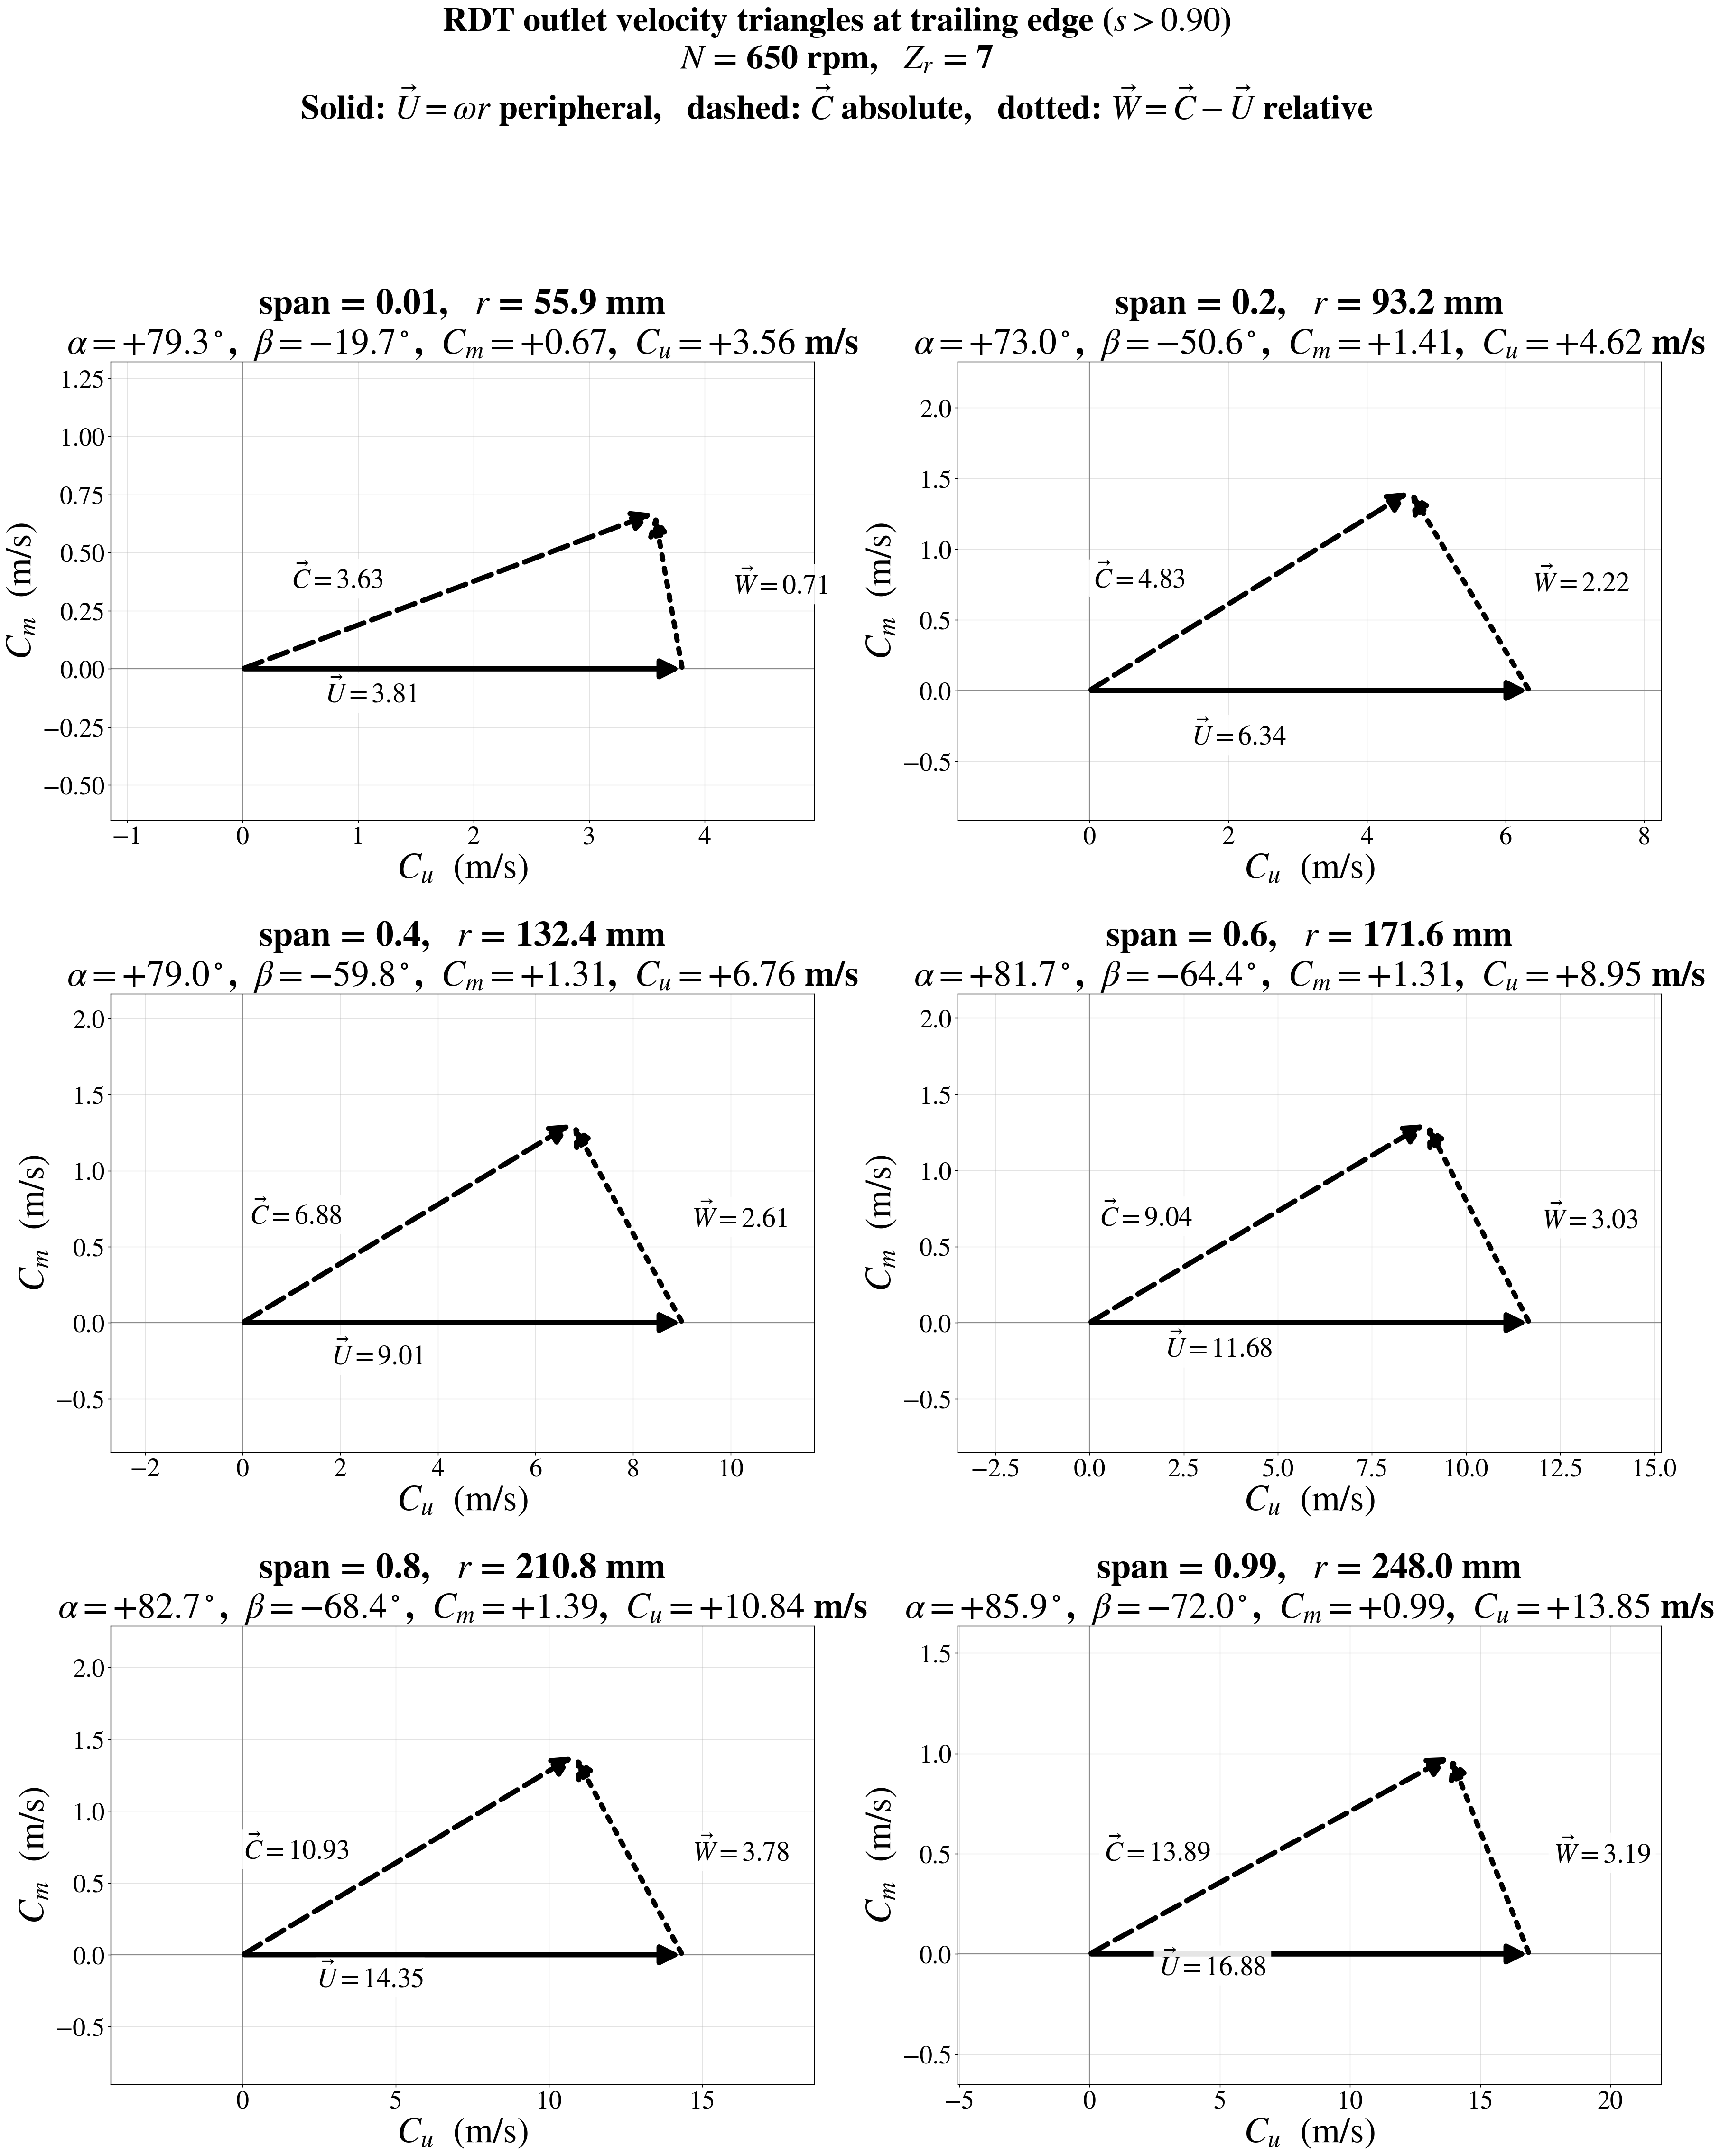
\includegraphics[width=0.99\linewidth]{Figures/RDT/RDT_velocity_triangles_TE.png}
%   \caption[Velocity triangles at the RDT trailing edge]{Velocity
%   triangles at the RDT trailing edge ($s>0.90$) for the six radial
%   spans used to characterise the wake. Blue: absolute velocity
%   $\vec{C}$; green: peripheral velocity $\vec{U}=\omega r$; red:
%   relative velocity $\vec{W}=\vec{C}-\vec{U}$. The three vectors close
%   as $\vec{C}=\vec{U}+\vec{W}$ by construction. Operating point:
%   $N=650$~rpm, $Z_r=7$. Sign convention follows
%   \eqref{eq:rdt_sign_convention}.}
%   \label{fig:rdt_velocity_triangles_TE}
% \end{figure}
 
% \paragraph{Near-leading-edge values: complementary diagnostic.}
% Figure~\ref{fig:rdt_velocity_triangles_LE} presents the velocity
% triangles constructed from the same blade-loading exports but evaluated
% in the near-LE window $s\in[0.05,\,0.15]$, after the LE
% stagnation/suction-peak spike has decayed and before the main
% chord-loaded region develops. Table~\ref{tab:rdt_le_values} summarises
% the corresponding components. These values describe the kinematic state
% of the flow on the rotor blade surface near the leading edge; they are
% \emph{not} the free-stream inlet velocity to the rotor. A free-stream
% inlet velocity would require a constant-$z$ plane export upstream of
% the rotor and is left to a follow-up post-processing step.
 
% \begin{table}[H]
%   \centering
%   \caption[RDT near-LE velocity triangle at six spans]{Velocity-triangle
%   components in the near-LE region ($s\in[0.05,\,0.15]$) of the RDT
%   blade-loading lines. Reported as a complementary diagnostic of the
%   kinematic state on the blade surface near the leading edge. These
%   values are not used as guide-vane design input. Sign convention as
%   in~\eqref{eq:rdt_sign_convention}.}
%   \label{tab:rdt_le_values}
%   \begin{tabular}{ccccccccc}
%     \hline
%     span & $r$ & $U$ & $C_m$ & $C_u$ & $W_u$ & $|\vec{C}|$ & $\alpha$ & $\beta$ \\
%          & [mm] & [m/s] & [m/s] & [m/s] & [m/s] & [m/s] & [$^\circ$] & [$^\circ$] \\
%     \hline
%     0.01 &  55.9 &  3.81 & $-1.51$ &  6.63 & $+2.82$ &  6.80 & $+102.8$ & $+118.1$ \\
%     0.20 &  93.2 &  6.34 &   0.37  &  4.80 & $-1.55$ &  4.81 &  $+85.6$ &  $-76.7$ \\
%     0.40 & 132.4 &  9.01 &   1.40  &  4.88 & $-4.13$ &  5.08 &  $+74.0$ &  $-71.3$ \\
%     0.60 & 171.6 & 11.68 &   2.23  &  6.27 & $-5.41$ &  6.66 &  $+70.5$ &  $-67.6$ \\
%     0.80 & 210.8 & 14.35 &   1.84  &  8.30 & $-6.05$ &  8.50 &  $+77.5$ &  $-73.1$ \\
%     0.99 & 248.0 & 16.88 &   0.16  & 10.88 & $-6.00$ & 10.89 &  $+89.2$ &  $-88.5$ \\
%     \hline
%   \end{tabular}
% \end{table}
 
% \begin{figure}[H]
%   \centering
%   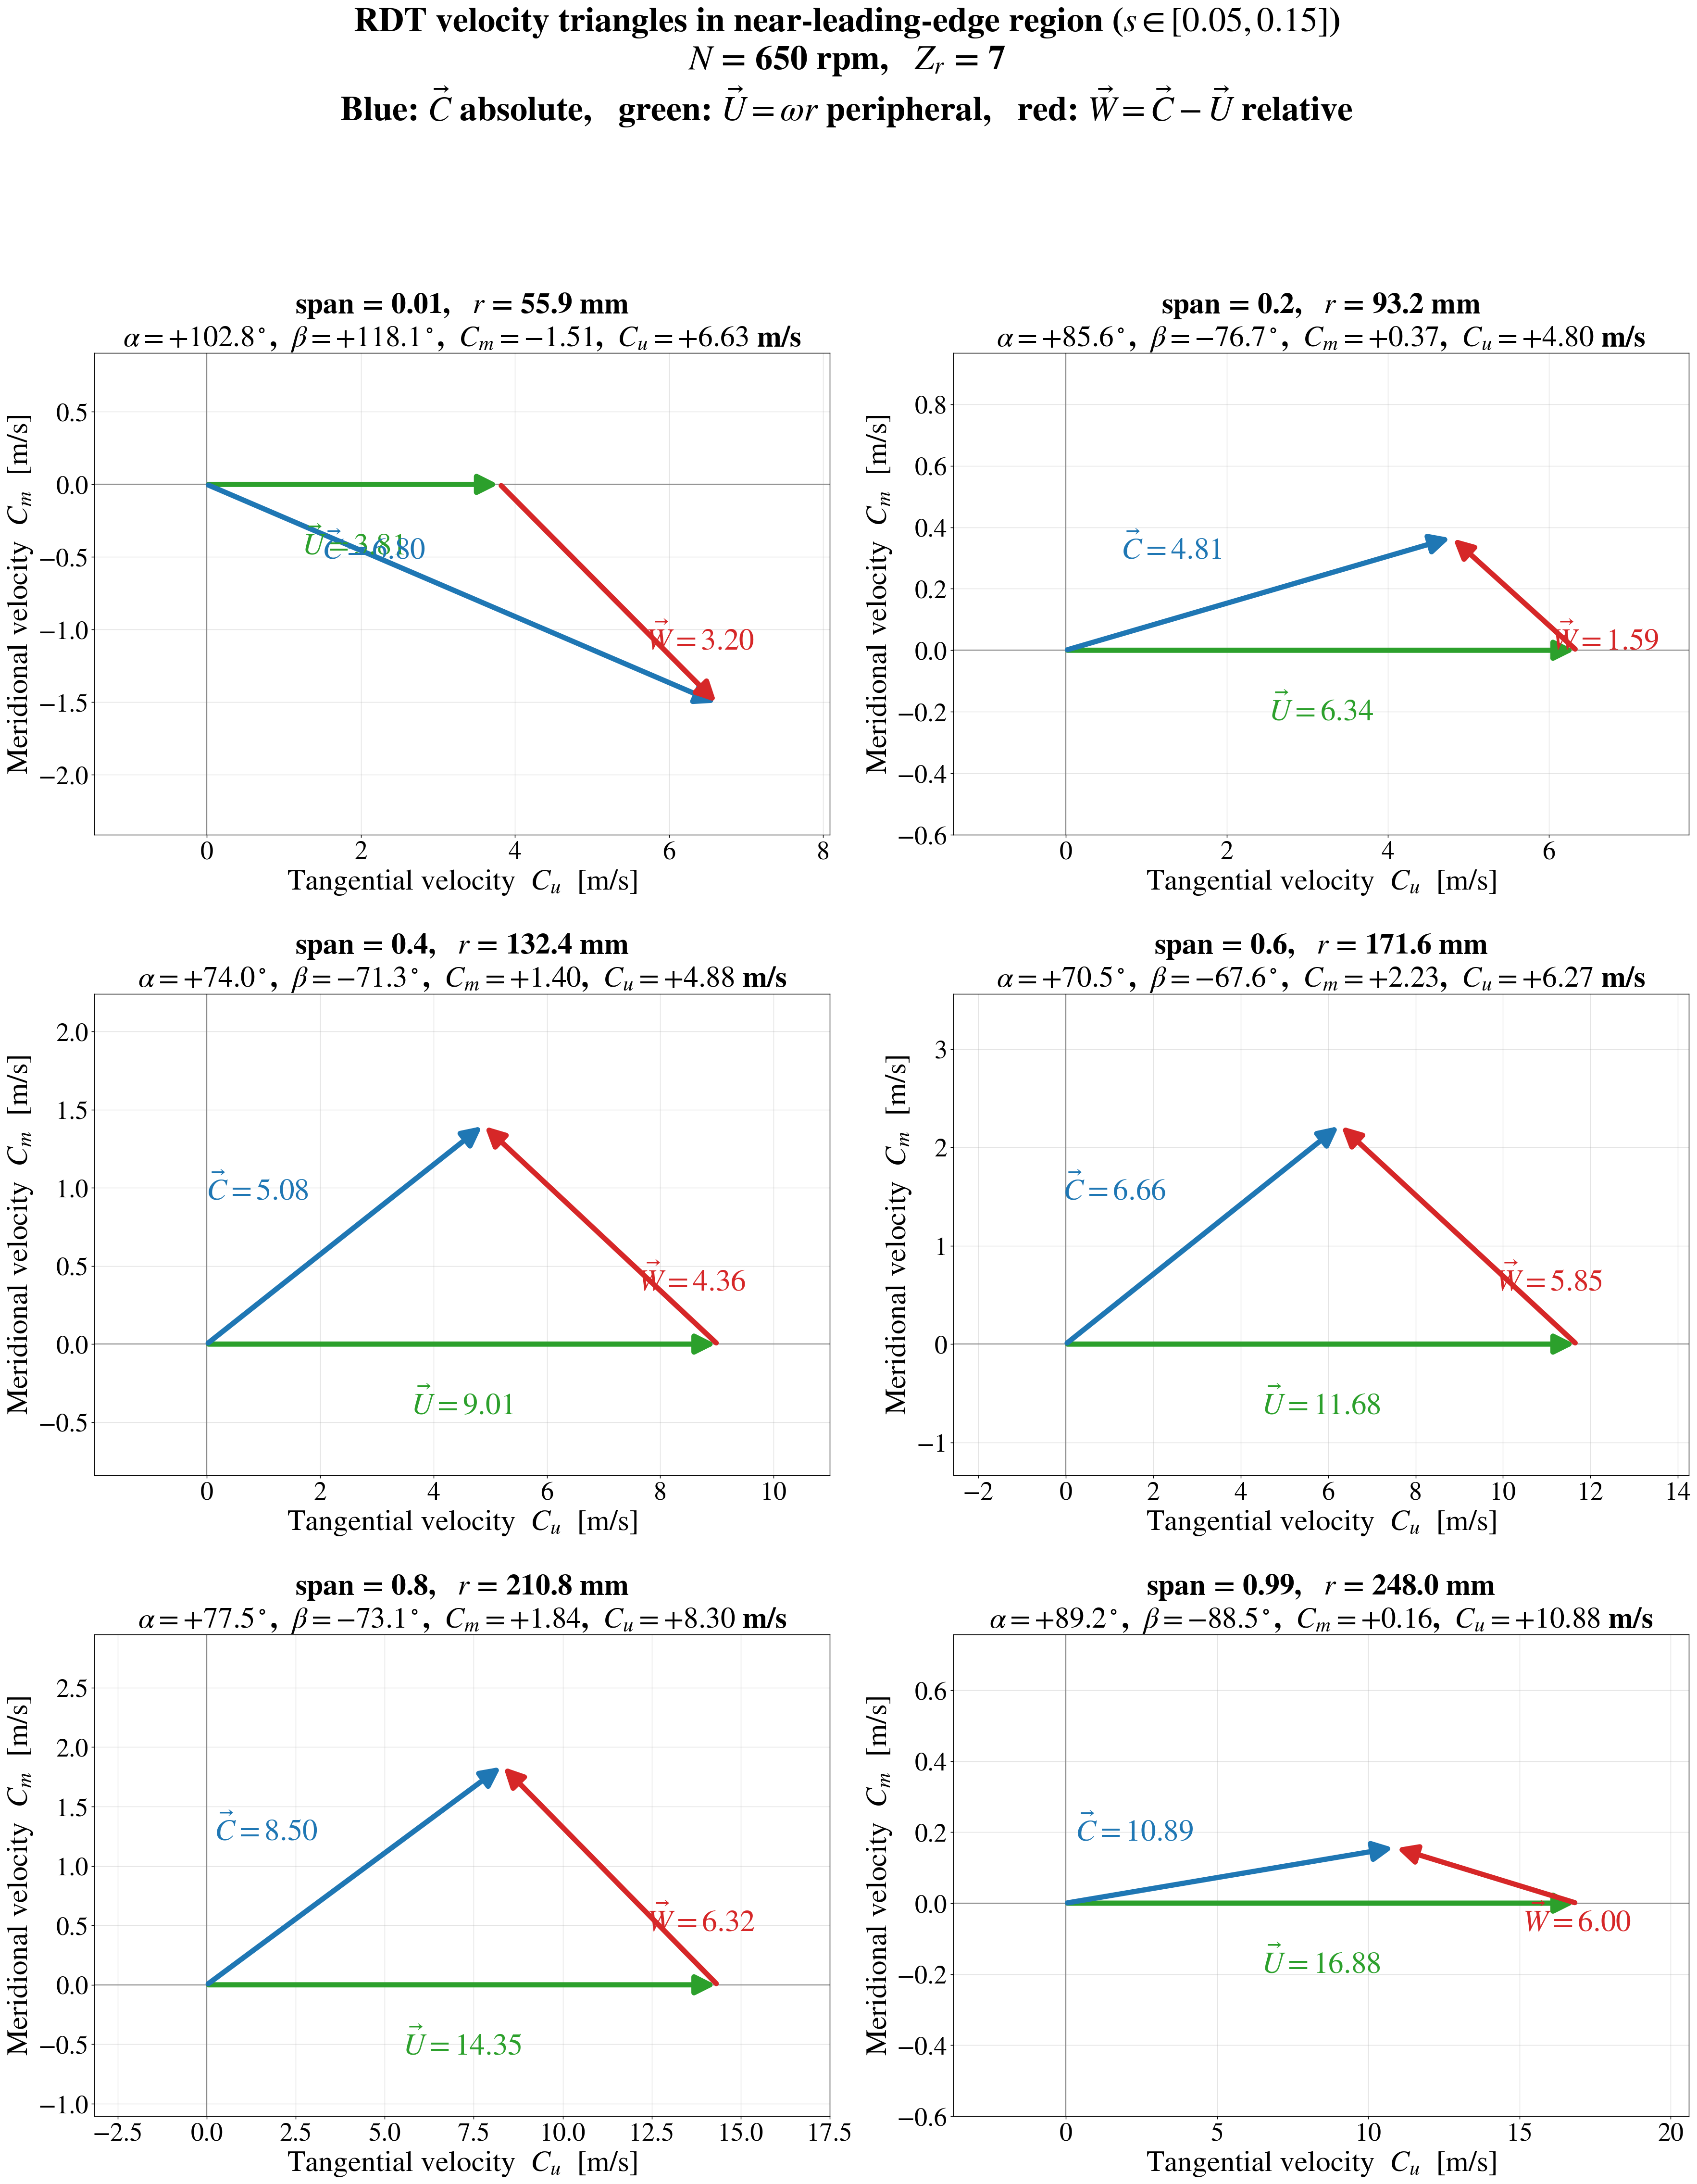
\includegraphics[width=0.99\linewidth]{Figures/RDT/RDT_velocity_triangles_LE.png}
%   \caption[Velocity triangles in the near-LE region of the RDT]{Velocity
%   triangles in the near-leading-edge region ($s\in[0.05,\,0.15]$) of the
%   RDT blade-loading lines for the six radial spans. Same layout and
%   vector convention as Figure~\ref{fig:rdt_velocity_triangles_TE}. The
%   span-$0.01$ panel exhibits a negative $C_m$, reflecting the proximity
%   of the LE stagnation/suction-peak structure on the blade surface near
%   the hub rather than a physical reverse free-stream condition.}
%   \label{fig:rdt_velocity_triangles_LE}
% \end{figure}
 
% \paragraph{Comparison of LE and TE regions.}
% Comparing Tables~\ref{tab:rdt_te_values} and~\ref{tab:rdt_le_values} and
% Figures~\ref{fig:rdt_velocity_triangles_TE}--\ref{fig:rdt_velocity_triangles_LE}
% provides physical insight into how the rotor blade does work on the
% flow as it traverses the chord. Three points are worth noting.
 
% First, the tangential component $C_u$ in the central span band
% ($r/R\in[0.40,\,0.80]$) is roughly $30$--$40\%$ smaller in the near-LE
% region than in the TE region (e.g.\ $4.88$~m/s vs.\ $6.76$~m/s at
% $r/R=0.40$; $8.30$~m/s vs.\ $10.84$~m/s at $r/R=0.80$). This
% qualitatively reflects the blade adding tangential momentum to the
% flow as it passes from LE to TE, which is consistent with the rotor
% acting as a pump in the absolute frame. The interpretation is
% qualitative because both samples are taken on the blade surface itself,
% not at upstream and downstream stations in the free stream.
 
% Second, the meridional component $C_m$ behaves differently in the two
% regions. In the TE region, $C_m$ is nearly uniform across the central
% span band, with a hub-side and a tip-side drop. In the near-LE region,
% $C_m$ is smaller at all spans, drops to $0.16$~m/s at $r/R=0.99$, and
% becomes \emph{negative} at $r/R=0.01$. A negative $C_m$ at $r/R=0.01$
% should not be interpreted as a physical reverse axial flow in the duct;
% it reflects the local boundary-layer and stagnation structure on the
% hub-side of the blade surface near the LE, where the blade-loading line
% samples the deceleration in the immediate vicinity of the leading-edge
% stagnation point. This is a known artefact of evaluating velocity on a
% blade surface and does not propagate to the free-stream wake.
 
% Third, the relative angle $\beta$ in the near-LE region is consistent
% with a strongly negative incidence at the inner spans, where $|\beta|$
% exceeds $70^\circ$ for $r/R\geq 0.40$. This is qualitatively consistent
% with the strong turning required of the rotor blades, which is
% ultimately what produces the high tangential velocity observed in the
% TE region. The near-LE diagnostic should therefore be read as a
% description of the loading regime on the blade surface rather than as
% an independent measurement of the upstream inflow.
 
% \paragraph{Limitations of the present wake characterisation.}
% The values in Tables~\ref{tab:rdt_te_values}--\ref{tab:rdt_le_values}
% are sampled on the blade surface at two streamwise windows of the
% blade-loading line. They are therefore most useful as relative
% indicators rather than as absolute measurements of the free-stream
% field. A constant-$z$ plane export downstream of the rotor (typically
% $0.5$--$1$ chord lengths downstream of the TE) would yield a
% mass-flow-averaged wake profile $(C_m(r),\,C_u(r))$ that is closer to
% the input format expected by the guide-vane generator and would also
% permit a direct Euler check against the design head of the rotor. This
% post-processing step is a planned refinement that does not affect the
% configurations selected for the screening campaign, since the guide-vane
% geometries already generated from the present TE values can be
% re-evaluated against an updated wake without altering the case matrix.

% \section{Pressure-coefficient distribution along the RDT blade}
% \label{sec:methods_rdt_cp}
 
% In addition to the velocity-triangle characterisation in
% Section~\ref{sec:methods_rdt_velocity_triangles}, the converged RDT-only
% solution is post-processed for the pressure distribution along the
% rotor blade contour at eleven radial spans, $r/R\in\{0.01,\,0.10,\,
% 0.20,\,0.30,\,\ldots,\,0.90,\,0.99\}$. The data are exported as
% blade-loading lines that traverse the blade contour
% $\mathrm{LE}\to\mathrm{SS}\to\mathrm{TE}\to\mathrm{PS}\to\mathrm{LE}$,
% where SS denotes the suction side and PS the pressure side. The
% streamwise coordinate $s\in[0,1]$ is normalised along the chord. Both
% surfaces appear naturally as the two branches of the same continuous
% contour line.
 
% \paragraph{Pressure-coefficient definition.}
% The static pressure $p$ is non-dimensionalised at each radius by the
% dynamic pressure based on the local blade speed,
% %
% \begin{equation}
% C_p(s,\,r) \;=\; \frac{p(s,\,r) - p_{\mathrm{ref}}}
%                        {\frac{1}{2}\,\rho\,U^{2}(r)},
% \qquad
% U(r) \;=\; \omega\,r,
% \label{eq:Cp_definition}
% \end{equation}
% %
% where $\omega$ is the rotor angular velocity and $\rho$ the water
% density. The reference pressure $p_{\mathrm{ref}}$ is the median
% pressure across all spans and all chord positions of the converged
% solution; this is a robust free-stream-like reference that makes the
% $C_p$ profiles directly comparable across spans without privileging any
% single radial location. With this scaling, $C_p$ is bounded near $-1$
% and $+1$ in the inner-mid-span region for a well-formed pump rotor, and
% positive (negative) values indicate static pressure above (below) the
% reference.
 
% \paragraph{Distribution at eleven spans.}
% Figure~\ref{fig:rdt_cp_distribution} shows $C_p(s)$ for all eleven
% spans, grouped by radial position into a hub-region panel
% ($r/R\leq 0.30$), a mid-span panel ($0.40\leq r/R\leq 0.70$), and a
% tip-region panel ($r/R\geq 0.80$). Three distinct regimes are visible.
 
% \begin{figure}[H]
%   \centering
%   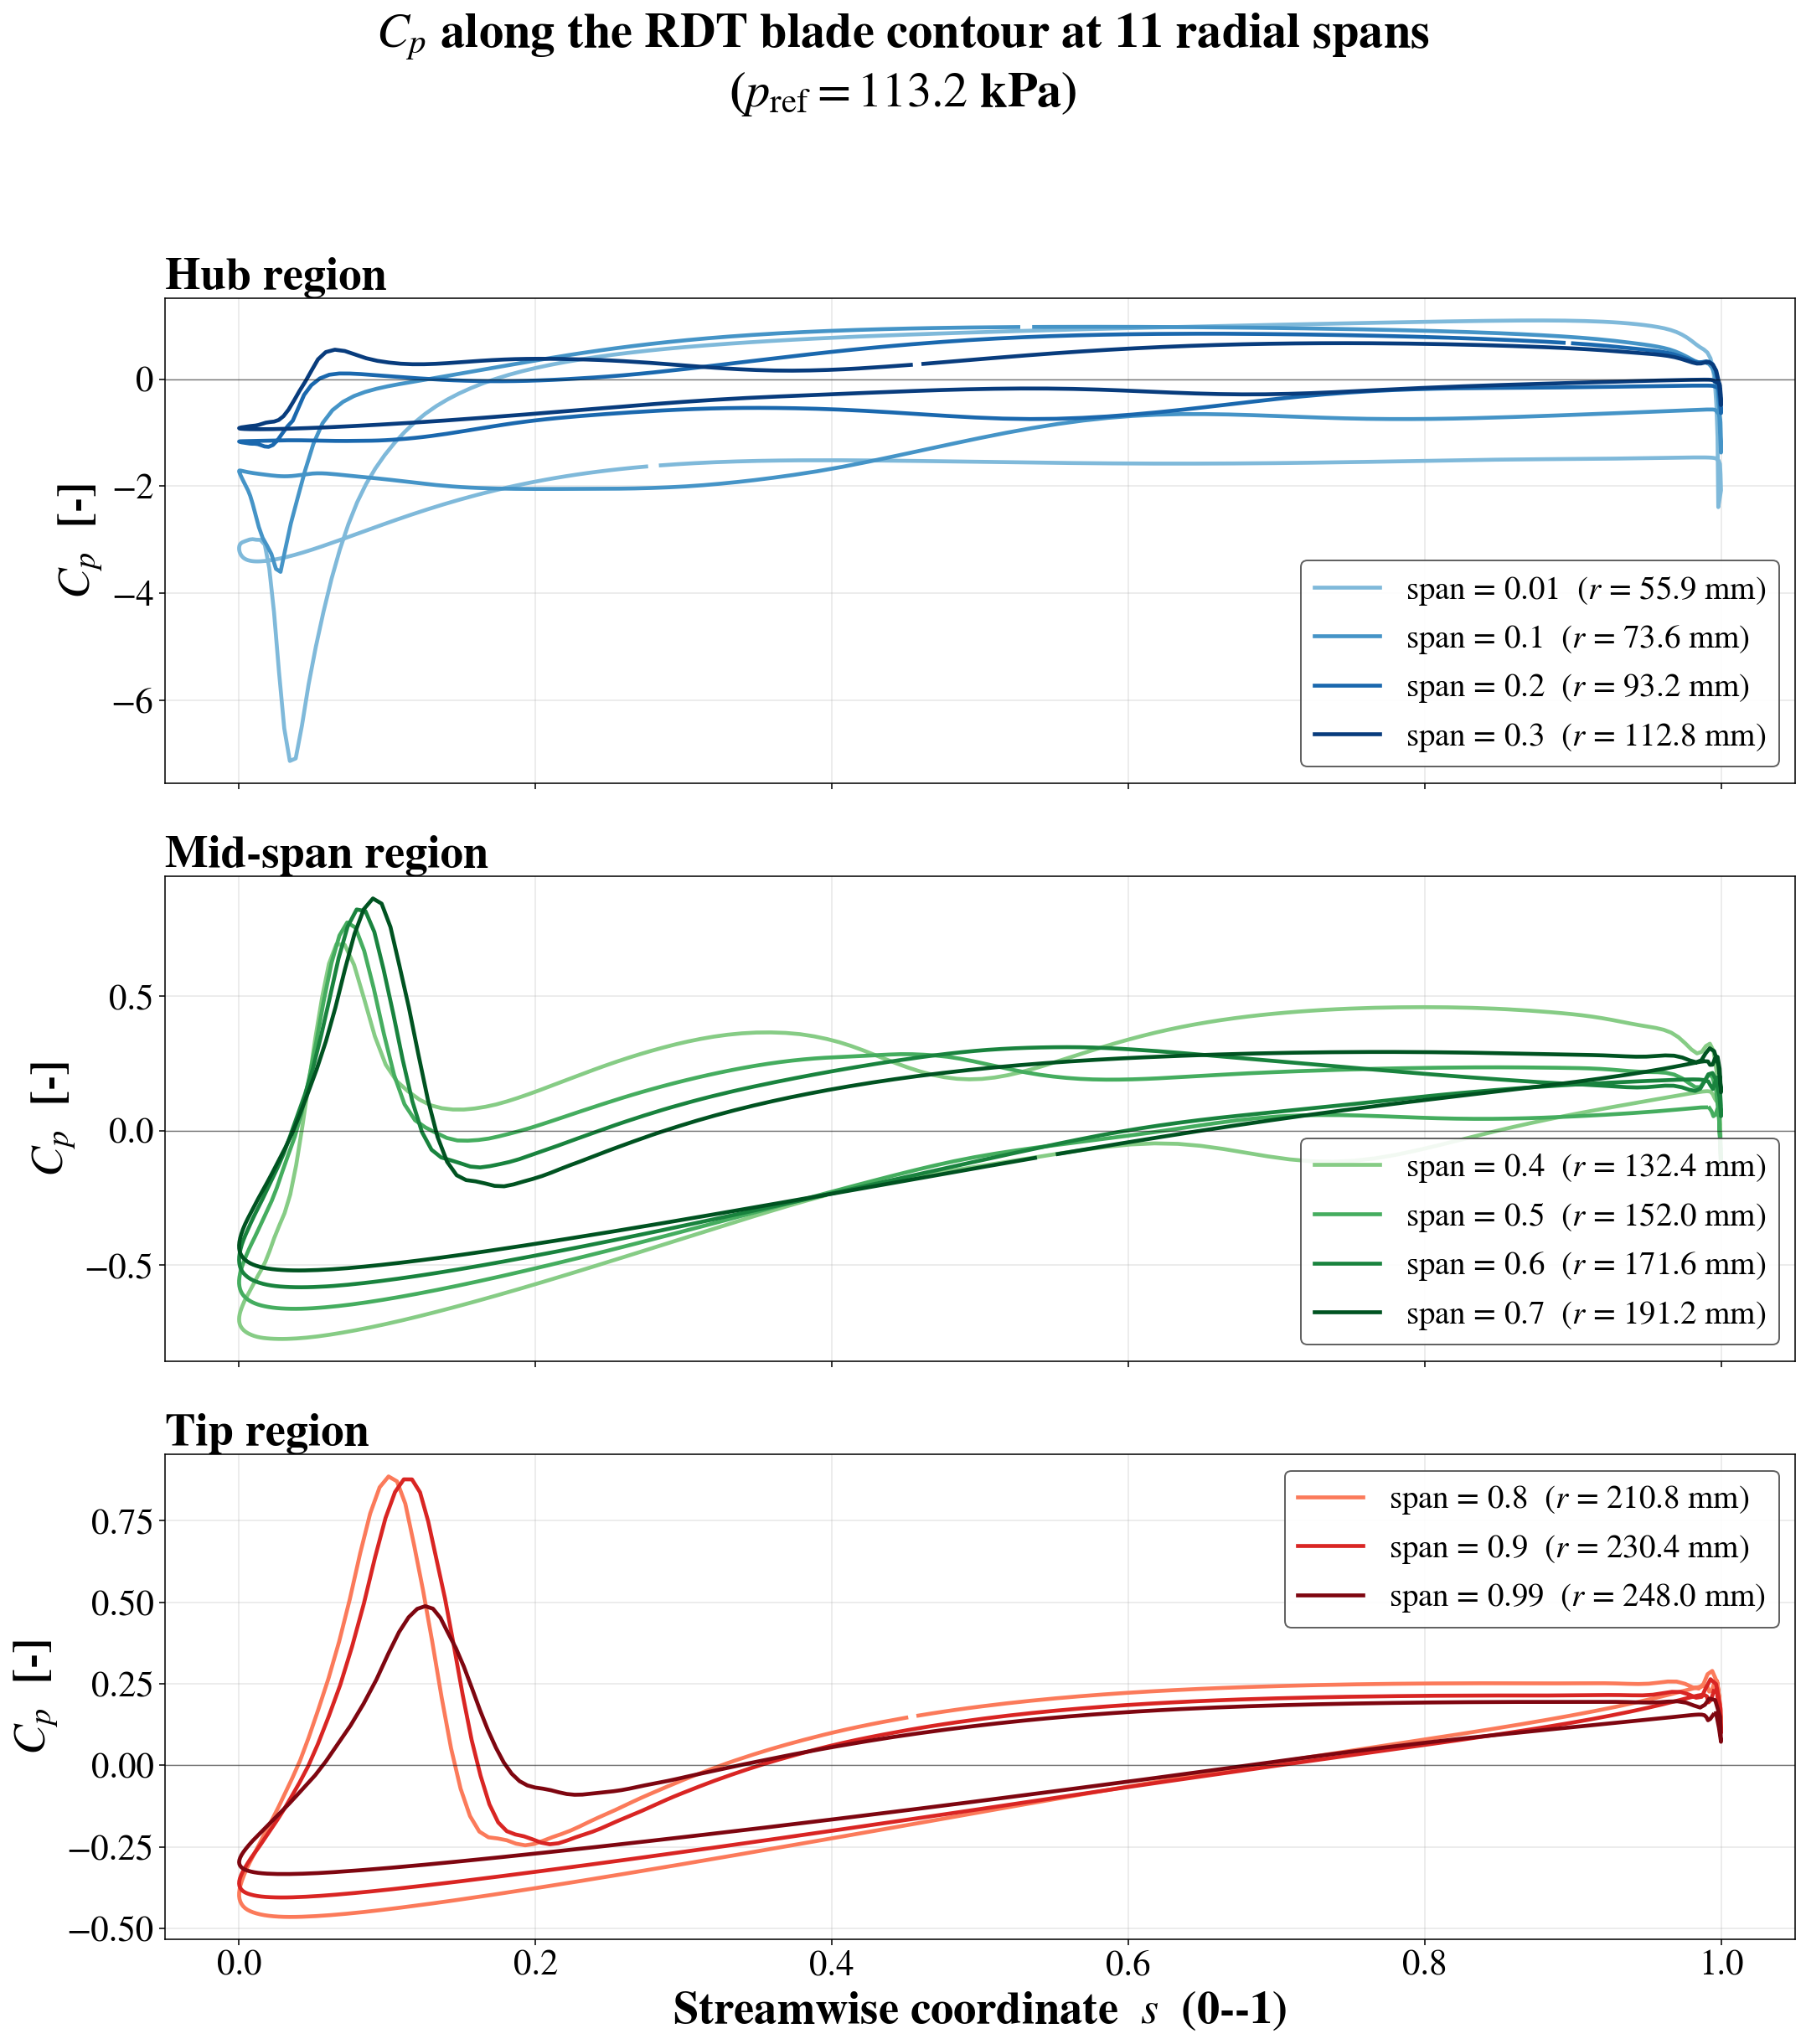
\includegraphics[width=\linewidth]{Figures/RDT/Spanwise_Cp_RDT.png}
%   \caption[Pressure-coefficient distribution along the RDT blade]
%   {Pressure coefficient $C_p$ along the RDT blade contour at eleven
%   radial spans. Each curve is a single continuous traversal of the
%   blade contour
%   $\mathrm{LE}\to\mathrm{SS}\to\mathrm{TE}\to\mathrm{PS}\to\mathrm{LE}$;
%   the two visible branches at every $s$ correspond to the suction
%   side (lower $C_p$) and the pressure side (higher $C_p$). The
%   reference pressure is the median pressure across all spans,
%   $p_{\mathrm{ref}}=113.2$~kPa. The grouping is hub
%   ($r/R\leq 0.30$, top), mid-span ($0.40\leq r/R\leq 0.70$, middle),
%   and tip ($r/R\geq 0.80$, bottom). The hub panel uses a different
%   vertical scale than the mid-span and tip panels because of the
%   large suction peak at $r/R=0.01$.}
%   \label{fig:rdt_cp_distribution}
% \end{figure}
 
% \paragraph{Hub region (top panel).}
% The innermost station, $r/R=0.01$, exhibits a deep suction peak with
% $C_p\approx -7$ near $s\approx 0.05$ and an essentially absent
% pressure-side loading. This indicates strong local acceleration around
% the blade leading edge in the immediate hub vicinity, consistent with
% high local incidence and with the absence of an actual hub solid body
% in this hubless rim-driven thruster~\cite{Verdijck2025}. Moving outward
% to $r/R=0.10,\,0.20$ and $0.30$, the suction peak weakens rapidly and
% the pressure side becomes increasingly identifiable, but a clean
% PS--SS separation is only consistently established from
% $r/R\gtrsim 0.30$ onwards. The hub region is therefore the part of the
% RDT outflow where the blade-loading concept itself is least
% representative of an aerofoil-like cascade. This observation is
% consistent with the backflow-dominated rings identified at
% $r<0.12$~m in the convergence analysis of
% Section~\ref{sec:methods_rdt_baseline_alpha} and provides a physical
% justification for the inner cut-out at $r=0.12$~m used in the
% guide-vane design span: the hub region delivers a flow that is
% dominated by recirculation rather than by a coherent rotor wake that
% the guide vanes can usefully condition.
 
% \paragraph{Mid-span region (middle panel).}
% The four mid-span stations, $r/R\in\{0.40,\,0.50,\,0.60,\,0.70\}$,
% display the classical pump-rotor blade-loading shape. The pressure side
% exhibits a localised peak of $C_p\approx +0.7$--$+0.9$ near
% $s\approx 0.10$, the suction side reaches a minimum of
% $C_p\approx -0.5$--$-0.7$ at the same chord location, and both surfaces
% recover smoothly through the diffusion region towards a near-zero
% $C_p$ at the trailing edge. The PS--SS separation is well-defined and
% the loading area enclosed between the two branches is large, indicating
% that this part of the blade does most of the useful pumping work. The
% absence of a flat or rising suction-side recovery suggests that no
% significant boundary-layer separation develops on the SS in the
% mid-span region under the present design point.
 
% \paragraph{Tip region (bottom panel).}
% At $r/R\in\{0.80,\,0.90\}$ the qualitative shape of the loading is the
% same as the mid-span, but the suction peak intensifies further with
% radius. The peak suction-side magnitude reaches $C_p\approx -0.4$ and
% the peak pressure-side value rises to $C_p\approx +0.9$ at
% $r/R=0.80$--$0.90$, which is consistent with the larger blade speed
% $U(r)=\omega r$ at the outer span and with the higher local relative
% velocity. At the outermost station, $r/R=0.99$, however, the loading
% drops noticeably: the PS--SS branches collapse towards each other and
% the enclosed loading area shrinks. The tip-vortex flow and the
% finite tip-clearance treatment unload the blade locally, in a manner
% that is well documented for ducted thrusters and pump
% rotors~\cite{Verdijck2025}. This unloading produces the
% characteristic outer-radius dip in $\alpha(r)$ that the baseline
% construction in
% Section~\ref{sec:methods_rdt_baseline_alpha} replaces with a
% $60^\circ$ plateau, since designing the guide-vane outer-span metal
% angle against this tip-driven feature would couple the vane geometry
% to a feature of the rotor that is not part of the swirl pattern the
% guide-vane row is intended to recover.
 
% \paragraph{Implications for the guide-vane design.}
% Three implications follow from Figure~\ref{fig:rdt_cp_distribution} and
% are used in the GV-design choices made in
% Section~\ref{sec:methods_design_matrix}. First, the breakdown of the
% blade-loading concept at $r/R\lesssim 0.20$ supports the choice of an
% inner cut-out at $r=0.12$~m: there is no coherent rotor outflow inside
% that radius for the guide vanes to recover. Second, the existence of a
% clean PS--SS pump-rotor loading from $r/R\gtrsim 0.30$ outward confirms
% that the swirl distribution $C_u(r)$ obtained from the converged plane
% is generated by a healthy, well-attached rotor and is not an artefact
% of off-design separation; the spanwise design input
% $(C_m(r),\,C_u(r))$ is therefore a meaningful target for the guide-vane
% generator. Third, the tip-vortex unloading at $r/R\approx 0.99$
% provides the physical justification for the plateau-bounded baseline
% $\alpha_{\mathrm{base}}(r)$ used in
% Section~\ref{sec:methods_rdt_baseline_alpha}: the local outer-radius
% dip in $\alpha(r)$ originates in the tip-clearance flow rather than in
% the bulk wake, and the guide-vane row should not be designed to track
% it.








% \section{Baseline guide-vane design profile from the converged RDT wake}
% \label{sec:methods_rdt_baseline_alpha}
 
% The blade-loading-line analysis in
% Section~\ref{sec:methods_rdt_velocity_triangles} characterises the
% kinematic state of the flow on the rotor blade trailing edge. For the
% guide-vane design the relevant input is, however, the radial profile of
% the absolute flow angle on a constant-$z$ plane downstream of the rotor,
% since this is the surface from which the guide-vane row receives its
% inflow. A separate post-processing step is therefore performed on a
% constant-$z$ plane extracted at $z=-0.185$~m, i.e.\ $0.185$~m downstream
% of the RDT centre, using the converged final time-window of the
% transient RDT-only simulation. This section documents how the spanwise
% design profile $\alpha_{\mathrm{base}}(r)$ is constructed from that
% plane and how its convergence is verified.
 
% \subsection{Plane definition and ring-wise mass-flow weighting}
 
% At each iteration export, the plane data are read as point-wise records
% of $(x,\,y,\,z,\,r,\,u,\,v,\,w)$ in the stationary frame. The
% meridional and tangential components are recovered from a cylindrical
% decomposition,
% %
% \begin{equation}
% C_m(r,\theta) \;=\; -w(r,\theta), \qquad
% C_u(r,\theta) \;=\; -u(r,\theta)\sin\theta + v(r,\theta)\cos\theta,
% \label{eq:plane_decomposition}
% \end{equation}
% %
% with the same sign convention as in~\eqref{eq:rdt_sign_convention}:
% $C_m>0$ is the streamwise direction and $C_u>0$ is the rotor rotation
% direction. Each point is assigned to a radial ring of width
% $\Delta r = 5$~mm. The mass-flow-weighted absolute flow angle in the
% ring is
% %
% \begin{equation}
% \alpha(r) \;=\; \mathrm{atan2}\!\Bigl(\overline{|C_u|}^{\,m},\;
%                                       \overline{|C_m|}^{\,m}\Bigr),
% \label{eq:alpha_ring_mflow}
% \end{equation}
% %
% where overbars denote mass-flow-weighted averages over the ring. The
% positive mass-flux summed across the plane is rescaled so that the
% total positive mass-flux exactly matches the inlet boundary condition,
% $\dot m = 290.3$~kg/s, ensuring that small numerical mass-conservation
% errors at the rotor-stationary interface do not contaminate the angle
% profile. A ring is flagged as \emph{backflow-dominated} when its
% integrated negative-$C_m$ mass-flux exceeds five per cent of the total
% mass-flux through that ring.
 
% \subsection{Convergence of the angle profile across the transient run}
 
% Eleven plane snapshots from the second half of the transient run are
% inspected, distributed from $t=0.898$~s ($\mathrm{iter}=7000$) to
% $t=2.126$~s ($\mathrm{iter}=14000$). Figure~\ref{fig:BaselinePlot1}
% shows the resulting $\alpha(r)$ over the full radial range
% $0\leq r\leq 0.25$~m for all eleven snapshots. The grey-shaded region
% $r<0.12$~m identifies the inner cut-out where no guide vane is placed;
% within this region the dashed segments mark rings that are
% backflow-dominated. The hub-side recirculation is a characteristic
% feature of the hubless rim-driven thruster~\cite{Verdijck2025} and is
% not part of the guide-vane design problem. Figure~\ref{fig:BaselinePlot2}
% restricts the radial axis to the active guide-vane design span
% $r\in[0.12,\,0.25]$~m on a refined vertical scale. The first snapshot
% ($t=0.898$~s) has not yet converged in shape and underestimates the
% hub-region peak by approximately $10^\circ$, while the remaining ten
% snapshots covering $t\in[1.026,\,2.126]$~s reproduce the same
% characteristic shape: a hub-region peak of $\alpha\approx 84^\circ$ at
% $r=0.12$~m, a monotone decrease through the design mid-span, a local
% dip near $r\approx 0.21$~m driven by the tip-vortex acceleration, and a
% recovery towards $\alpha\approx 75^\circ$ at the outer wall. The
% spread between the converged snapshots is below approximately
% $2^\circ$ across the design span, which is sufficient for a
% single-curve baseline to be defined.
 
% \begin{figure}[H]
%   \centering
%   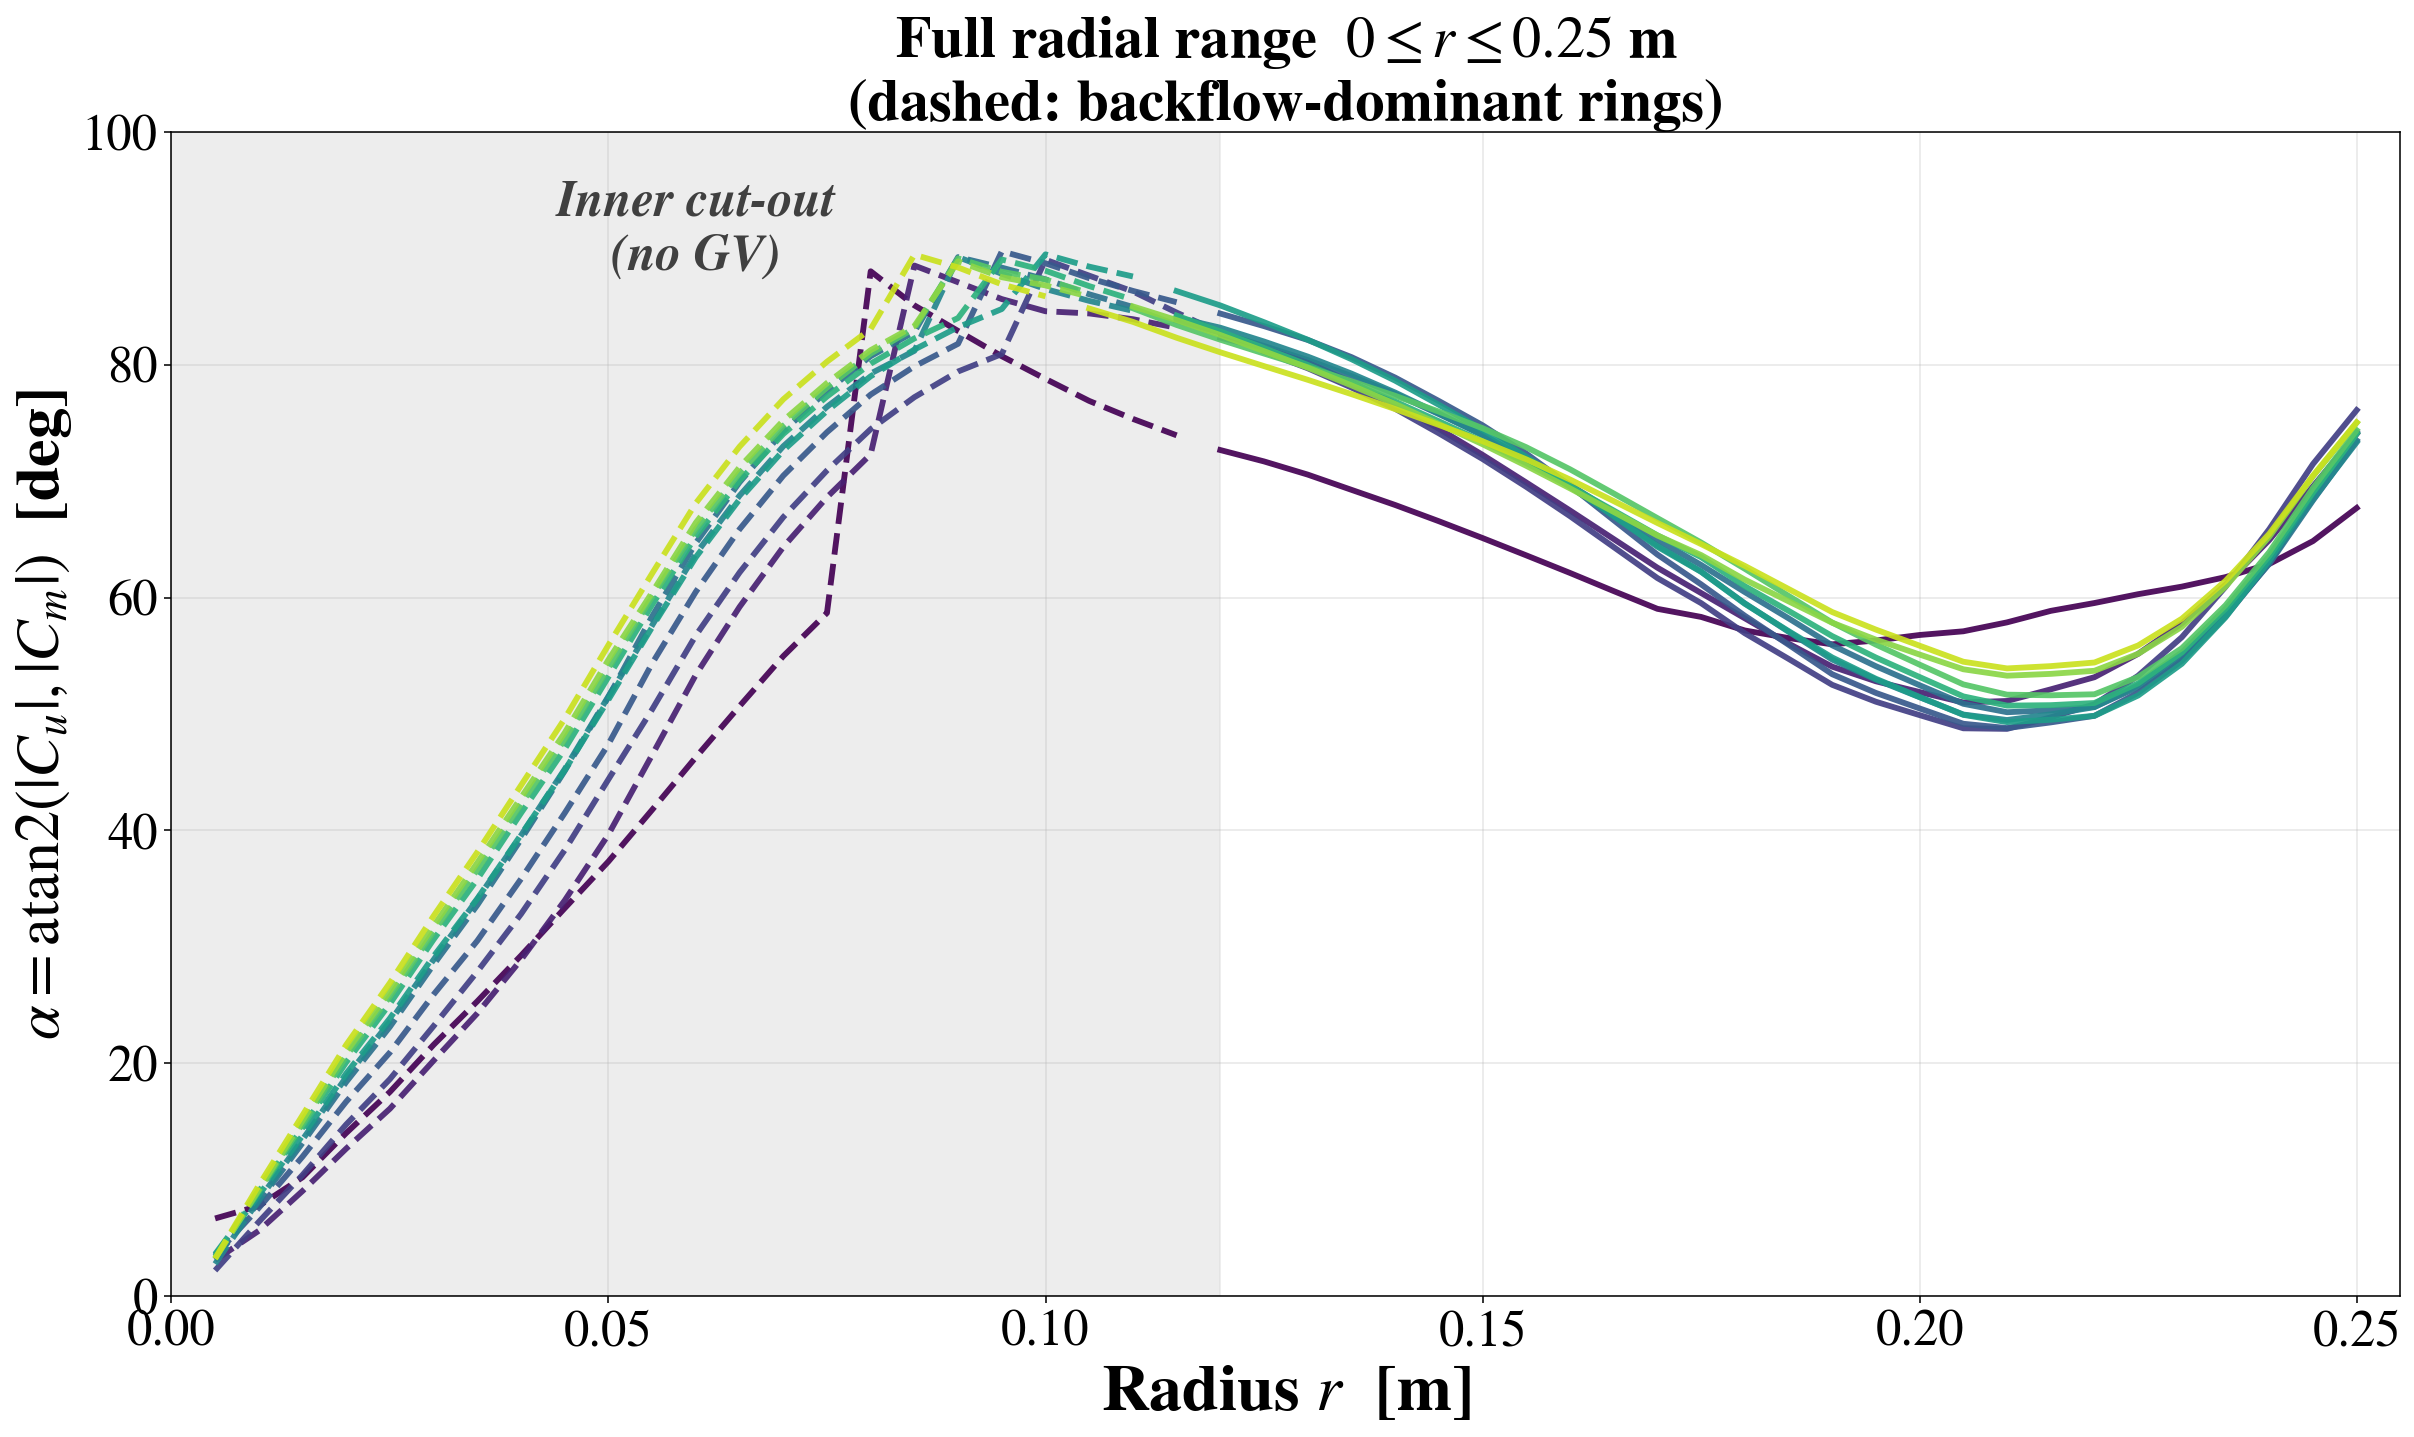
\includegraphics[width=\linewidth]{Figures/Methods/BaselinePlot1.png}
%   \caption[Convergence of $\alpha(r)$ at the RDT outlet plane, full range]
%   {Absolute flow angle $\alpha(r)$ at the RDT outlet plane
%   ($z=-0.185$~m) over eleven snapshots in the second half of the
%   transient run. The grey-shaded region $r<0.12$~m is the inner cut-out
%   where no guide vane is placed; dashed segments indicate
%   backflow-dominated rings (integrated negative-$C_m$ mass-flux above
%   five per cent). The hub-side recirculation is characteristic of the
%   hubless rim-driven thruster and is not part of the guide-vane design
%   problem.}
%   \label{fig:BaselinePlot1}
% \end{figure}
 
% \begin{figure}[H]
%   \centering
%   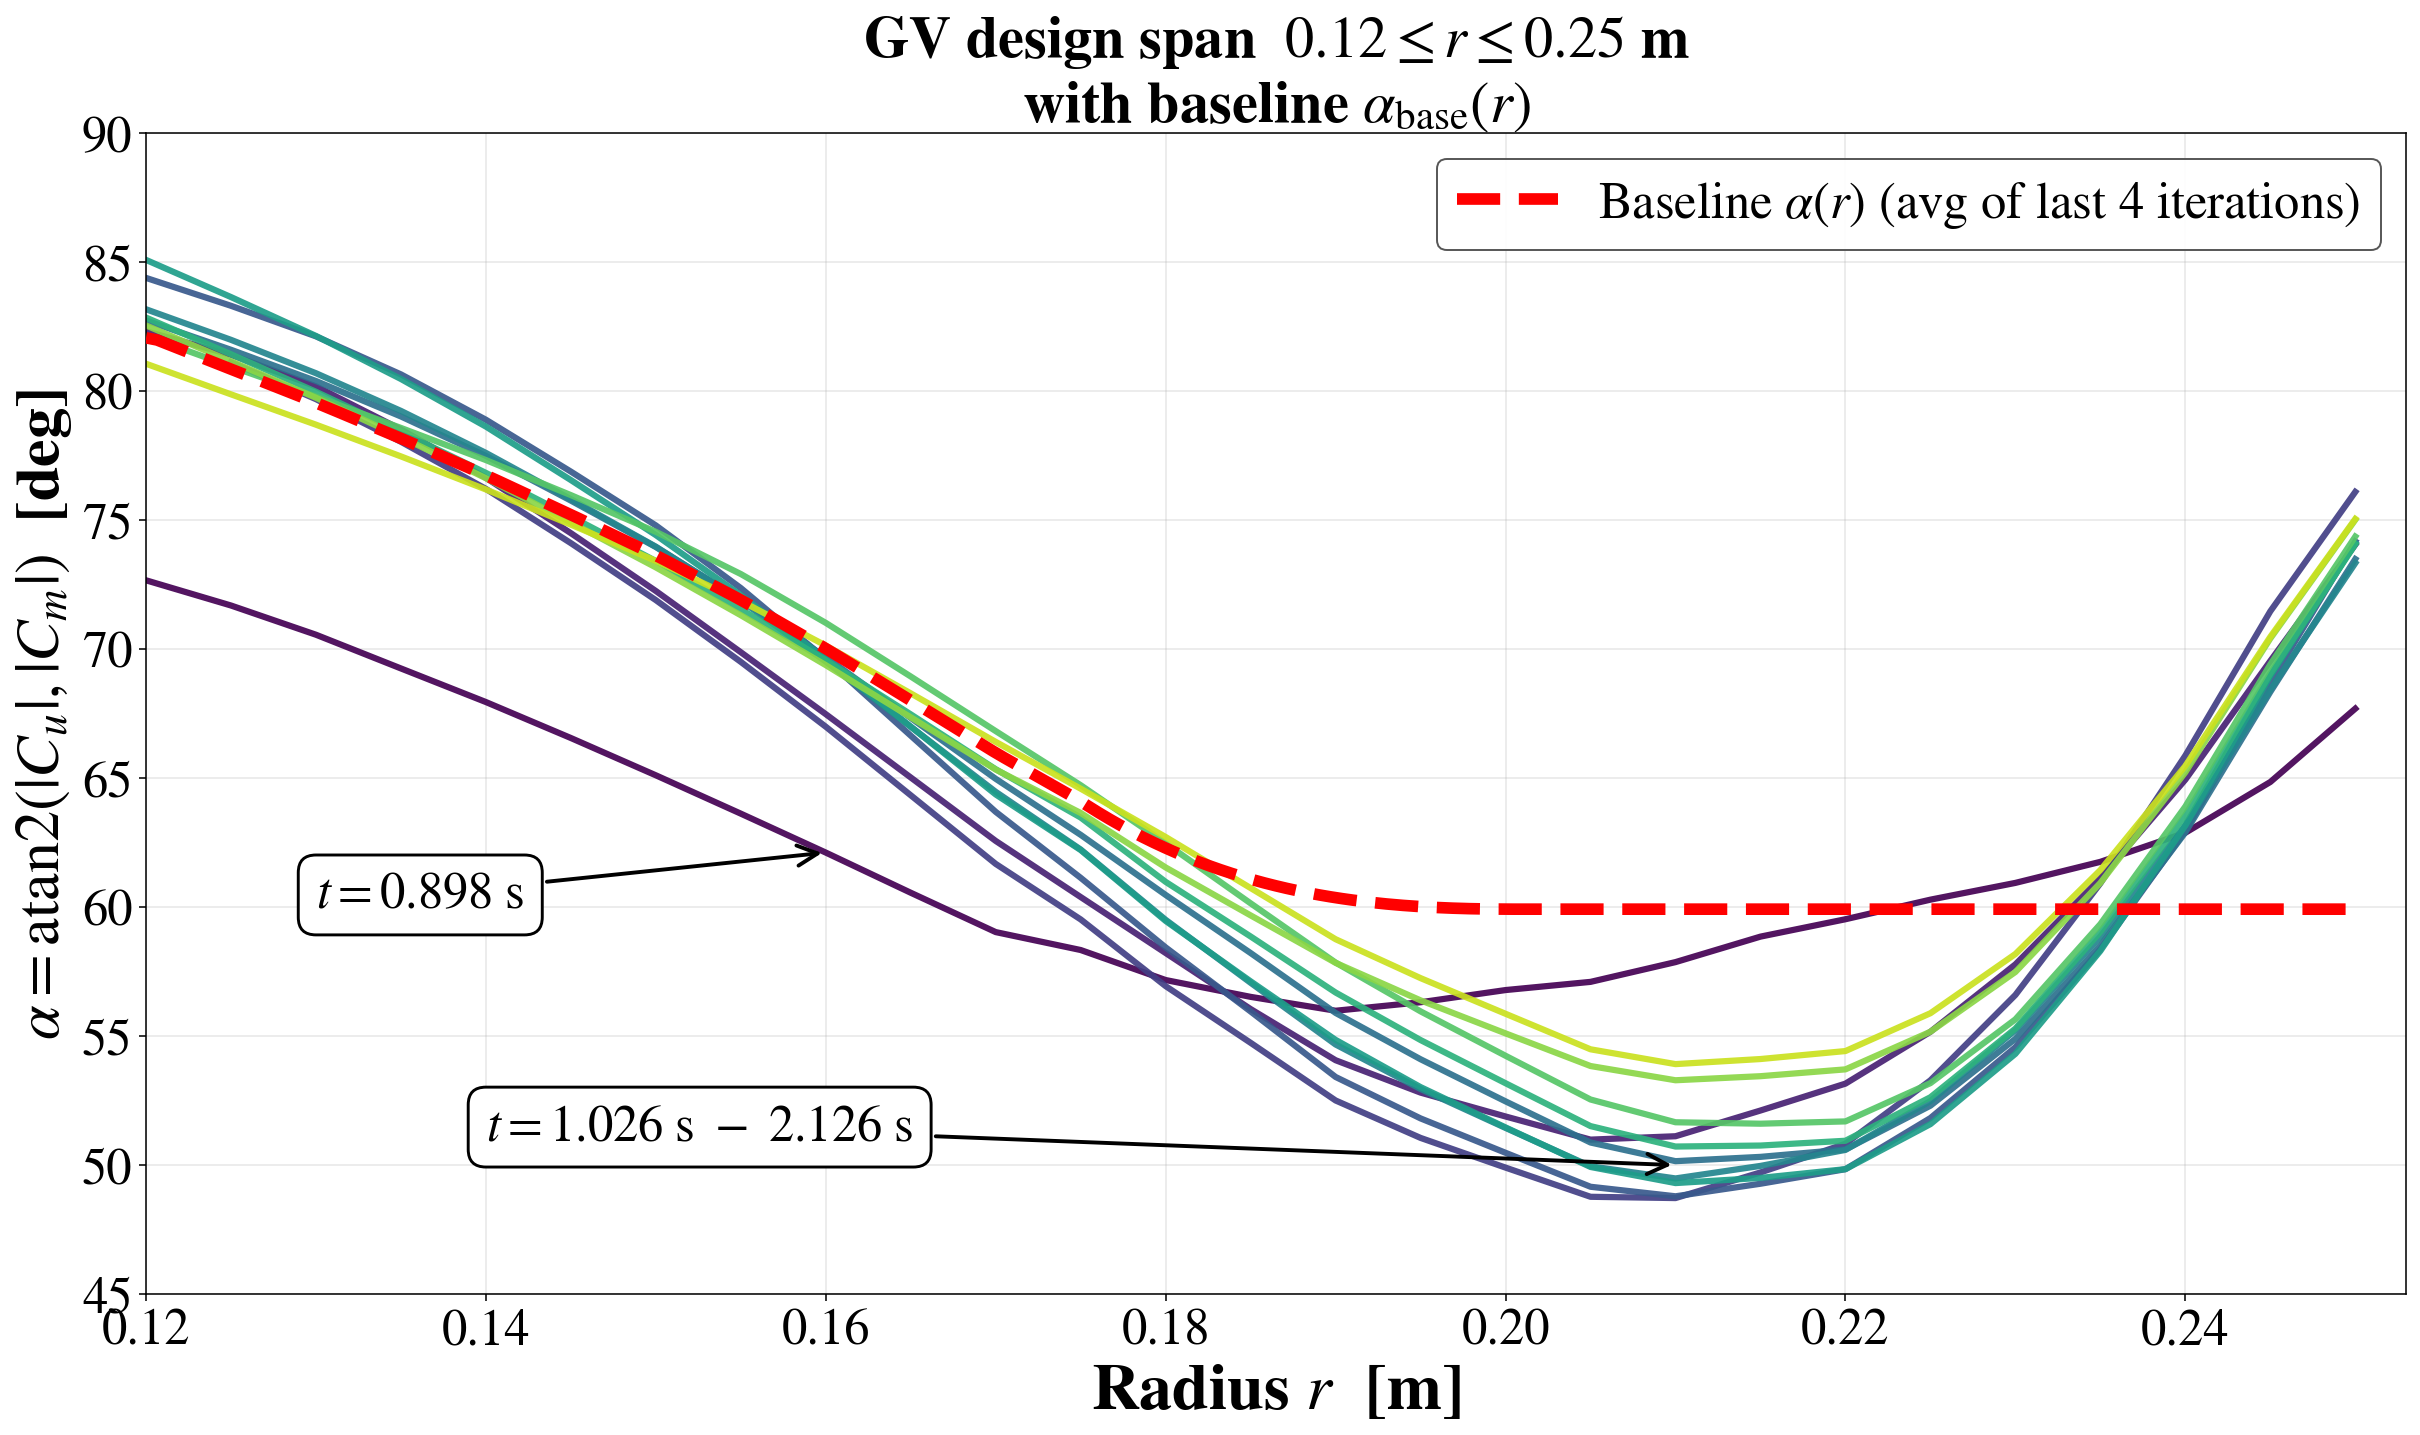
\includegraphics[width=\linewidth]{Figures/Methods/BaselinePlot2.png}
%   \caption[Baseline $\alpha(r)$ for guide-vane design, GV span only]
%   {Absolute flow angle $\alpha(r)$ in the active guide-vane design span
%   $r\in[0.12,\,0.25]$~m. The first transient snapshot
%   ($t=0.898$~s) has not yet converged in shape; the remaining ten
%   snapshots ($t\in[1.026,\,2.126]$~s) reproduce a stable angle profile
%   with a spread below approximately $2^\circ$. The constructed baseline
%   $\alpha_{\mathrm{base}}(r)$ (red dashed line) is the smoothed
%   monotone profile fitted to the average of the last four converged
%   snapshots, blended onto a $60^\circ$ outer plateau. This baseline is
%   the spanwise design input passed to the guide-vane generator for both
%   the constant-solidity and the constant-chord families in
%   Section~\ref{sec:methods_design_matrix}.}
%   \label{fig:BaselinePlot2}
% \end{figure}
 
% \subsection{Construction of the design baseline $\alpha_{\mathrm{base}}(r)$}
 
% Since the converged spread across snapshots is small but not zero, the
% baseline used as guide-vane design input is constructed as a smoothed
% monotone profile fitted to the average of the last four converged
% exports
% ($\mathrm{iter}\in\{12500,\,13000,\,13500,\,14000\}$, corresponding to
% $t\in[1.741,\,2.126]$~s). The procedure has five steps:
% \begin{enumerate}
% \item Average the four converged $\alpha(r)$ profiles on a common
%       radial grid by linear interpolation, producing
%       $\overline{\alpha}(r)$ on $r\in[0.12,\,0.25]$~m.
% \item Smooth $\overline{\alpha}(r)$ with a centred moving-mean filter
%       of width five points to suppress small ring-to-ring noise.
% \item Enforce a non-increasing envelope by sweeping outward and
%       clipping any local rise; this is a physical regularity
%       constraint, since the absolute angle is expected to decrease
%       monotonically from a tangential-dominated hub region towards a
%       more meridional outer region.
% \item Identify the curve-bend radius $r_{\mathrm{bend}}$ as the smallest
%       radius at which the monotone profile drops below the threshold
%       $\alpha_{\mathrm{bend}}=64^\circ$, and define a plateau target
%       $\alpha_{\mathrm{plateau}}=60^\circ$ for the outer span.
% \item Replace the profile in the transition region
%       $r\in[r_{\mathrm{bend}},\,r_{\mathrm{bend}}+\Delta r_{\mathrm{blend}}]$
%       with a cubic Hermite blend that matches the local slope of the
%       monotone average at $r_{\mathrm{bend}}$ and zero slope at
%       $r_{\mathrm{bend}}+\Delta r_{\mathrm{blend}}$, with
%       $\Delta r_{\mathrm{blend}}=35$~mm.
% \end{enumerate}
% The resulting baseline $\alpha_{\mathrm{base}}(r)$ is shown as a red
% dashed line in Figure~\ref{fig:BaselinePlot2}. The plateau choice
% $\alpha_{\mathrm{plateau}}=60^\circ$ is selected slightly above the
% local outer-radius dip ($\sim$~$50$--$54^\circ$) seen in the snapshot
% data. Designing the guide-vane leading-edge metal angle directly
% against this dip would lock the vane geometry to a peripheral flow
% feature that is sensitive to the rotor tip-clearance treatment and that
% the guide-vane row is not intended to track. The plateau therefore acts
% as a physically motivated upper envelope of the outer-span angle.
 
% \subsection{Spanwise design input passed to the guide-vane generator}
 
% Two spanwise quantities are required as input to the guide-vane generator: $\alpha_{\mathrm{base}}(r)$ as derived above, and a reference $C_m(r)$ used to recover $C_u(r) = C_m(r)\,\tan\alpha_{\mathrm{base}}(r)$. The reference $C_m(r)$ is the mass-flow-weighted average of the same last four converged exports on the same radial grid as the baseline. This procedure produces a triplet $\bigl(r,\,C_m(r),\,C_u(r)\bigr)$ that is internally consistent with $\alpha_{\mathrm{base}}(r)$ at every radius. The discrete spanwise input is sampled at fifty equally spaced radii in $r\in[0.12,\,0.25]$~m. Selected rows are listed in Table~\ref{tab:rdt_baseline_gv_input}; the full 50-point dataset is provided in the accompanying digital file \texttt{baseline\_gv\_input.csv}. Both the constant-solidity and the constant-chord guide-vane families described in Section~\ref{sec:methods_design_matrix} are designed against this single baseline so that all 24 configurations face an identical inflow specification, and any difference in their performance is attributable to chord, vane count, and turning choices alone.
 
% \begin{table}[H]
%   \centering
%   \caption[Selected rows of the baseline GV design input]{Selected rows of the baseline guide-vane design input $\bigl(r,\,\alpha_{\mathrm{base}},\,C_m,\,C_u\bigr)$ used as the spanwise specification for both the constant-solidity and the constant-chord guide-vane families. The full 50-point dataset is available in \texttt{baseline\_gv\_input.csv}. Sign convention follows
%   \eqref{eq:rdt_sign_convention}.}
%   \label{tab:rdt_baseline_gv_input}
%   \begin{tabular}{rrrr}
%     \hline
%     $r$ [m] & $\alpha_{\mathrm{base}}$ [$^\circ$] & $C_m$ [m/s] & $C_u$ [m/s] \\
%     \hline
%     0.120  & 83.8 & 0.512 & 4.699 \\
%     0.140  & 77.7 & 1.008 & 4.622 \\
%     0.160  & 71.0 & 1.501 & 4.364 \\
%     0.180  & 63.0 & 2.078 & 4.085 \\
%     0.200  & 59.9 & 2.821 & 4.856 \\
%     0.220  & 59.9 & 3.046 & 5.259 \\
%     0.240  & 59.9 & 2.674 & 4.620 \\
%     0.250  & 59.9 & 1.854 & 3.201 \\
%     \hline
%   \end{tabular}
% \end{table}
 
% \subsection{Connection to the trailing-edge velocity triangles}
 
% The hub-region peak of $\alpha\approx 84^\circ$ at $r=0.12$~m and the outer-span values around $\alpha\approx 60^\circ$ in the present constant-$z$ plane are consistent with the trailing-edge values reported in Table~\ref{tab:rdt_te_values}, which give $\alpha\approx 79^\circ$ at $r/R=0.40$ rising to $\sim 86^\circ$ at $r/R=0.99$. The blade-loading-line samples in Section~\ref{sec:methods_rdt_velocity_triangles} characterise the local kinematic state at the rotor blade trailing edge, while the constant-$z$ plane sample used here characterises the wake the guide vane actually sees. The two are physically related but not identical: the angle on the blade surface near the TE reflects the local turning imposed by the rotor blade, whereas the angle on the constant-$z$ plane reflects the developed wake after the local pressure-side and suction-side flows have merged. The design baseline uses the constant-$z$ plane angle because that is the physical surface from which the guide-vane row receives its inflow.
 
% \subsection{Why the baseline is smoothed and bounded}
 
% Three features of the raw converged profile justify the smoothed, plateau-bounded baseline rather than passing the average $\alpha(r)$ directly into the guide-vane generator. First, the noise envelope around the average profile is finite, on the order of $1$--$2^\circ$, and feeding this noise directly into the leading-edge metal-angle calculation would cause local oscillations in vane stagger that have no physical basis. Second, the outer-span dip ($\alpha\approx 50$--$54^\circ$ near $r\approx 0.21$~m) is driven by the tip-vortex-induced local acceleration at the rotor tip and is therefore tied to the rotor tip-clearance configuration; designing the guide-vane outer-span angle against this dip would couple the vane
% geometry to a rotor feature that is independent of the guide-vane row. Third, a monotone non-increasing $\alpha(r)$ matches the physical expectation that the absolute angle decreases from the swirl-dominated hub region towards a plateau region in the outer span. The plateau treatment is therefore both a noise-reduction step and a physical regularisation, and it does not affect the overall turning task that the guide vanes are designed to perform.
 